% Options for packages loaded elsewhere
\PassOptionsToPackage{unicode}{hyperref}
\PassOptionsToPackage{hyphens}{url}
%
\documentclass[
]{book}
\usepackage{amsmath,amssymb}
\usepackage{iftex}
\ifPDFTeX
  \usepackage[T1]{fontenc}
  \usepackage[utf8]{inputenc}
  \usepackage{textcomp} % provide euro and other symbols
\else % if luatex or xetex
  \usepackage{unicode-math} % this also loads fontspec
  \defaultfontfeatures{Scale=MatchLowercase}
  \defaultfontfeatures[\rmfamily]{Ligatures=TeX,Scale=1}
\fi
\usepackage{lmodern}
\ifPDFTeX\else
  % xetex/luatex font selection
\fi
% Use upquote if available, for straight quotes in verbatim environments
\IfFileExists{upquote.sty}{\usepackage{upquote}}{}
\IfFileExists{microtype.sty}{% use microtype if available
  \usepackage[]{microtype}
  \UseMicrotypeSet[protrusion]{basicmath} % disable protrusion for tt fonts
}{}
\makeatletter
\@ifundefined{KOMAClassName}{% if non-KOMA class
  \IfFileExists{parskip.sty}{%
    \usepackage{parskip}
  }{% else
    \setlength{\parindent}{0pt}
    \setlength{\parskip}{6pt plus 2pt minus 1pt}}
}{% if KOMA class
  \KOMAoptions{parskip=half}}
\makeatother
\usepackage{xcolor}
\usepackage{color}
\usepackage{fancyvrb}
\newcommand{\VerbBar}{|}
\newcommand{\VERB}{\Verb[commandchars=\\\{\}]}
\DefineVerbatimEnvironment{Highlighting}{Verbatim}{commandchars=\\\{\}}
% Add ',fontsize=\small' for more characters per line
\usepackage{framed}
\definecolor{shadecolor}{RGB}{248,248,248}
\newenvironment{Shaded}{\begin{snugshade}}{\end{snugshade}}
\newcommand{\AlertTok}[1]{\textcolor[rgb]{0.94,0.16,0.16}{#1}}
\newcommand{\AnnotationTok}[1]{\textcolor[rgb]{0.56,0.35,0.01}{\textbf{\textit{#1}}}}
\newcommand{\AttributeTok}[1]{\textcolor[rgb]{0.13,0.29,0.53}{#1}}
\newcommand{\BaseNTok}[1]{\textcolor[rgb]{0.00,0.00,0.81}{#1}}
\newcommand{\BuiltInTok}[1]{#1}
\newcommand{\CharTok}[1]{\textcolor[rgb]{0.31,0.60,0.02}{#1}}
\newcommand{\CommentTok}[1]{\textcolor[rgb]{0.56,0.35,0.01}{\textit{#1}}}
\newcommand{\CommentVarTok}[1]{\textcolor[rgb]{0.56,0.35,0.01}{\textbf{\textit{#1}}}}
\newcommand{\ConstantTok}[1]{\textcolor[rgb]{0.56,0.35,0.01}{#1}}
\newcommand{\ControlFlowTok}[1]{\textcolor[rgb]{0.13,0.29,0.53}{\textbf{#1}}}
\newcommand{\DataTypeTok}[1]{\textcolor[rgb]{0.13,0.29,0.53}{#1}}
\newcommand{\DecValTok}[1]{\textcolor[rgb]{0.00,0.00,0.81}{#1}}
\newcommand{\DocumentationTok}[1]{\textcolor[rgb]{0.56,0.35,0.01}{\textbf{\textit{#1}}}}
\newcommand{\ErrorTok}[1]{\textcolor[rgb]{0.64,0.00,0.00}{\textbf{#1}}}
\newcommand{\ExtensionTok}[1]{#1}
\newcommand{\FloatTok}[1]{\textcolor[rgb]{0.00,0.00,0.81}{#1}}
\newcommand{\FunctionTok}[1]{\textcolor[rgb]{0.13,0.29,0.53}{\textbf{#1}}}
\newcommand{\ImportTok}[1]{#1}
\newcommand{\InformationTok}[1]{\textcolor[rgb]{0.56,0.35,0.01}{\textbf{\textit{#1}}}}
\newcommand{\KeywordTok}[1]{\textcolor[rgb]{0.13,0.29,0.53}{\textbf{#1}}}
\newcommand{\NormalTok}[1]{#1}
\newcommand{\OperatorTok}[1]{\textcolor[rgb]{0.81,0.36,0.00}{\textbf{#1}}}
\newcommand{\OtherTok}[1]{\textcolor[rgb]{0.56,0.35,0.01}{#1}}
\newcommand{\PreprocessorTok}[1]{\textcolor[rgb]{0.56,0.35,0.01}{\textit{#1}}}
\newcommand{\RegionMarkerTok}[1]{#1}
\newcommand{\SpecialCharTok}[1]{\textcolor[rgb]{0.81,0.36,0.00}{\textbf{#1}}}
\newcommand{\SpecialStringTok}[1]{\textcolor[rgb]{0.31,0.60,0.02}{#1}}
\newcommand{\StringTok}[1]{\textcolor[rgb]{0.31,0.60,0.02}{#1}}
\newcommand{\VariableTok}[1]{\textcolor[rgb]{0.00,0.00,0.00}{#1}}
\newcommand{\VerbatimStringTok}[1]{\textcolor[rgb]{0.31,0.60,0.02}{#1}}
\newcommand{\WarningTok}[1]{\textcolor[rgb]{0.56,0.35,0.01}{\textbf{\textit{#1}}}}
\usepackage{longtable,booktabs,array}
\usepackage{calc} % for calculating minipage widths
% Correct order of tables after \paragraph or \subparagraph
\usepackage{etoolbox}
\makeatletter
\patchcmd\longtable{\par}{\if@noskipsec\mbox{}\fi\par}{}{}
\makeatother
% Allow footnotes in longtable head/foot
\IfFileExists{footnotehyper.sty}{\usepackage{footnotehyper}}{\usepackage{footnote}}
\makesavenoteenv{longtable}
\usepackage{graphicx}
\makeatletter
\def\maxwidth{\ifdim\Gin@nat@width>\linewidth\linewidth\else\Gin@nat@width\fi}
\def\maxheight{\ifdim\Gin@nat@height>\textheight\textheight\else\Gin@nat@height\fi}
\makeatother
% Scale images if necessary, so that they will not overflow the page
% margins by default, and it is still possible to overwrite the defaults
% using explicit options in \includegraphics[width, height, ...]{}
\setkeys{Gin}{width=\maxwidth,height=\maxheight,keepaspectratio}
% Set default figure placement to htbp
\makeatletter
\def\fps@figure{htbp}
\makeatother
\setlength{\emergencystretch}{3em} % prevent overfull lines
\providecommand{\tightlist}{%
  \setlength{\itemsep}{0pt}\setlength{\parskip}{0pt}}
\setcounter{secnumdepth}{5}
% definitions for citeproc citations
\NewDocumentCommand\citeproctext{}{}
\NewDocumentCommand\citeproc{mm}{%
  \begingroup\def\citeproctext{#2}\cite{#1}\endgroup}
\makeatletter
 % allow citations to break across lines
 \let\@cite@ofmt\@firstofone
 % avoid brackets around text for \cite:
 \def\@biblabel#1{}
 \def\@cite#1#2{{#1\if@tempswa , #2\fi}}
\makeatother
\newlength{\cslhangindent}
\setlength{\cslhangindent}{1.5em}
\newlength{\csllabelwidth}
\setlength{\csllabelwidth}{3em}
\newenvironment{CSLReferences}[2] % #1 hanging-indent, #2 entry-spacing
 {\begin{list}{}{%
  \setlength{\itemindent}{0pt}
  \setlength{\leftmargin}{0pt}
  \setlength{\parsep}{0pt}
  % turn on hanging indent if param 1 is 1
  \ifodd #1
   \setlength{\leftmargin}{\cslhangindent}
   \setlength{\itemindent}{-1\cslhangindent}
  \fi
  % set entry spacing
  \setlength{\itemsep}{#2\baselineskip}}}
 {\end{list}}
\usepackage{calc}
\newcommand{\CSLBlock}[1]{\hfill\break\parbox[t]{\linewidth}{\strut\ignorespaces#1\strut}}
\newcommand{\CSLLeftMargin}[1]{\parbox[t]{\csllabelwidth}{\strut#1\strut}}
\newcommand{\CSLRightInline}[1]{\parbox[t]{\linewidth - \csllabelwidth}{\strut#1\strut}}
\newcommand{\CSLIndent}[1]{\hspace{\cslhangindent}#1}
\usepackage{tikz-cd}
\usepackage{booktabs}
\usepackage{longtable}
\usepackage{array}
\usepackage{multirow}
\usepackage{wrapfig}
\usepackage{float}
\usepackage{colortbl}
\usepackage{pdflscape}
\usepackage{tabu}
\usepackage{threeparttable}
\usepackage{threeparttablex}
\usepackage[normalem]{ulem}
\usepackage{makecell}
\usepackage{xcolor}
\ifLuaTeX
  \usepackage{selnolig}  % disable illegal ligatures
\fi
\usepackage{bookmark}
\IfFileExists{xurl.sty}{\usepackage{xurl}}{} % add URL line breaks if available
\urlstyle{same}
\hypersetup{
  pdftitle={Fluent Graphics},
  pdfauthor={Adam Bartonicek},
  hidelinks,
  pdfcreator={LaTeX via pandoc}}

\title{Fluent Graphics}
\author{Adam Bartonicek}
\date{}

\begin{document}
\maketitle

{
\setcounter{tocdepth}{1}
\tableofcontents
}
\chapter{Abstract}\label{abstract}

Interactive data visualization has become a staple of modern data presentation. Yet, despite its growing popularity, there still exists many unresolved issues which make the process of producing rich interactive data visualizations difficult. Chief among these is the problem of data pipelines: how do we design a framework for turning raw data into summary statistics that can then be visualized, efficiently, on demand, and in a visually coherent way? Despite seeming like a straightforward task, there are in fact many subtle problems that arise when designing such a pipeline, and some of these may require a dramatic shift in perspective. In this thesis, I argue that, in order to design coherent generic interactive data visualization systems, we need to ground our thinking in concepts from some fairly abstract areas of mathematics including category theory and abstract algebra. By leveraging these algebraic concepts, we may be able to build more flexible and expressive interactive data visualization systems.

\newcommand\then{⨾}

\chapter{Introduction}\label{introduction}

\begin{quote}
It's written here: `In the Beginning was the Word!'
Here I stick already! Who can help me? It's absurd,
{[}\ldots{]}
The Spirit helps me! I have it now, intact.
And firmly write: 'In the Beginning was the Act!

Faust, Part I, Johann Wolfgang von Goethe (\citeproc{ref-goethe2015}{{[}1808{]} 2015})
\end{quote}

Humans are intensely visual creatures. About 20-30\% of our brain is involved in visual processing (\citeproc{ref-van2003}{Van Essen 2003}; \citeproc{ref-sheth2016}{Sheth and Young 2016}), utilizing a highly sophisticated and powerful visual processing pipeline (see e.g. \citeproc{ref-goebel2004}{Goebel, Muckli, and Kim 2004}; \citeproc{ref-knudsen2020}{Knudsen 2020}; for a brief review, see \citeproc{ref-ware2019}{Ware 2019}). It is well-established the brain can process certain salient visual stimuli in sub-20-millisecond times, outside of conscious attention (\citeproc{ref-ledoux2000}{LeDoux 2000}, \citeproc{ref-ledoux2003}{2003}), and that people can make accurate, parallel, and extremely rapid visual judgements, in phenomena known as subitizing and pre-attentive processing (\citeproc{ref-mandler1982}{Mandler and Shebo 1982}; \citeproc{ref-treisman1985}{Treisman 1985}). These features make the visual cortex the most powerful information channel that humans possess, both in terms of bandwidth and throughput.

Statisticians have known about this power of visual presentation for a long time. Starting with early charts and maps, data visualization co-evolved alongside mathematical statistics, offering an alternative and complementary perspective (for a review, see \citeproc{ref-friendly2006}{Friendly 2006} or Section \ref{brief-history}). While mathematical statistics tended to focus on confirmatory hypothesis testing, data visualization provided avenues for unsupervised exploration, ``forcing us to notice that which we would never expect to see'' (\citeproc{ref-tukey1977}{Tukey et al. 1977}). Eventually, this valuable role of forcing us to see the unexpected established data visualization as a respected tool within the applied statistician's toolkit.

Seeing an object from a distance is one thing, but being able to also touch, manipulate, and probe it is another. Within the human brain, action and perception are not independent, but are instead intricately linked, mutually reinforcing processes (see e.g. \citeproc{ref-dijkerman2007}{Dijkerman and De Haan 2007}; \citeproc{ref-lederman2009}{Lederman and Klatzky 2009}). Beginning in the 1970's, statisticians acquired a new set of tools for exploiting this connection. The advent of computer graphics and interactive data visualization transformed the idea of ``interrogating a chart'' from a mere turn of phrase into tangible reality. All of a sudden, it became possible to work with the visual representation of data in a tactile way, getting new perspectives and insights at the stroke of a key or click of a button.

This compelling union of the visual and the tactile has made interactive data visualization a popular method of presenting data. Nowadays, there are many packages and libraries for building interactive data visualizations across all the major data analytic languages. Interactive figures make frequent appearance in online news articles and commercial dashboards. However, despite this apparent popularity, significant gaps remain in the use and understanding of interactive visualizations. Individual analysts rarely utilize interactive data visualization tools (see e.g. \citeproc{ref-batch2017}{Batch and Elmqvist 2017}), the availability of certain more sophisticated interactive features is fairly limited (see Section \ref{litreview}), and researchers still point to a lack of a general interactive data visualization pipeline (\citeproc{ref-wickham2009}{Wickham et al. 2009}; \citeproc{ref-vanderplas2020}{Vanderplas, Cook, and Hofmann 2020}).

This thesis explores these interactive data visualization paradoxes and the inherent challenges surrounding interactive data visualization pipelines more specifically. I argue that, contrary to some prevailing views, interactivity is not simply an add-on to static graphics. Instead, interactive visualizations must be designed with interactivity as a primary consideration. Furthermore, I contend that certain interactive features fundamentally influence the types of visualizations that can be effectively presented. My claim is that popular types of interactive visualizations exhibit a particular kind congruence between graphics, statistics, and interaction, and that the absence of this congruence results in suboptimal visualizations. I formalize this congruence using the framework of category theory. Finally, I validate these theoretical concepts by developing an open-source interactive data visualization library and demonstrate its application to real-world data.

\subsubsection{Thesis Overview}\label{thesis-overview}

The thesis is organized as follows. Section \ref{litreview} reviews the history of interactive data visualization and discusses general trends and issues in the field. Section \ref{problems}, focuses on specific problems encountered when designing an interactive data visualization pipeline. Section \ref{goals}, outlines the the goals and aims that guided the development of the interactive data visualization library. Section \ref{system} details the system's components and design considerations. Section \ref{applied-example}, presents an applied example of exploring a real-world data set using the developed library. Finally, Section \ref{discussion}, discusses lessons learned and potential future research directions.

\chapter{Background}\label{litreview}

\section{Brief history of interactive data visualization}\label{brief-history}

Data visualization has a rich and intricate history, and a comprehensive treatment is beyond the scope of the present thesis. Nevertheless, in this section, I will provide a brief overview, with a particular focus on the later developments related to interactive visualization. For a more detailed historical account, readers should refer to Beniger and Robyn (\citeproc{ref-beniger1978}{1978}), Dix and Ellis (\citeproc{ref-dix1998}{1998}), Friendly (\citeproc{ref-friendly2006}{2006}), Friendly and Wainer (\citeproc{ref-friendly2021}{2021}), or Young, Valero-Mora, and Friendly (\citeproc{ref-young2011}{2011}).

\subsection{Static data visualization: From ancient times to the space age}\label{static-data-visualization-from-ancient-times-to-the-space-age}

The idea of graphically representing abstract information is very old. As one concrete example, a clay tablet recording a land survey during the Old Babylonian period (approximately 1900-1600 BCE) has recently been identified as the earliest visual depiction of the Pythagorean theorem (\citeproc{ref-mansfield2020}{Mansfield 2020}). Other examples of early abstract visualizations include maps of geographic regions and the night sky, and these were also the first to introduce the idea of coordinate systems (\citeproc{ref-beniger1978}{Beniger and Robyn 1978}; \citeproc{ref-friendly2021}{Friendly and Wainer 2021}).

\begin{figure}

{\centering 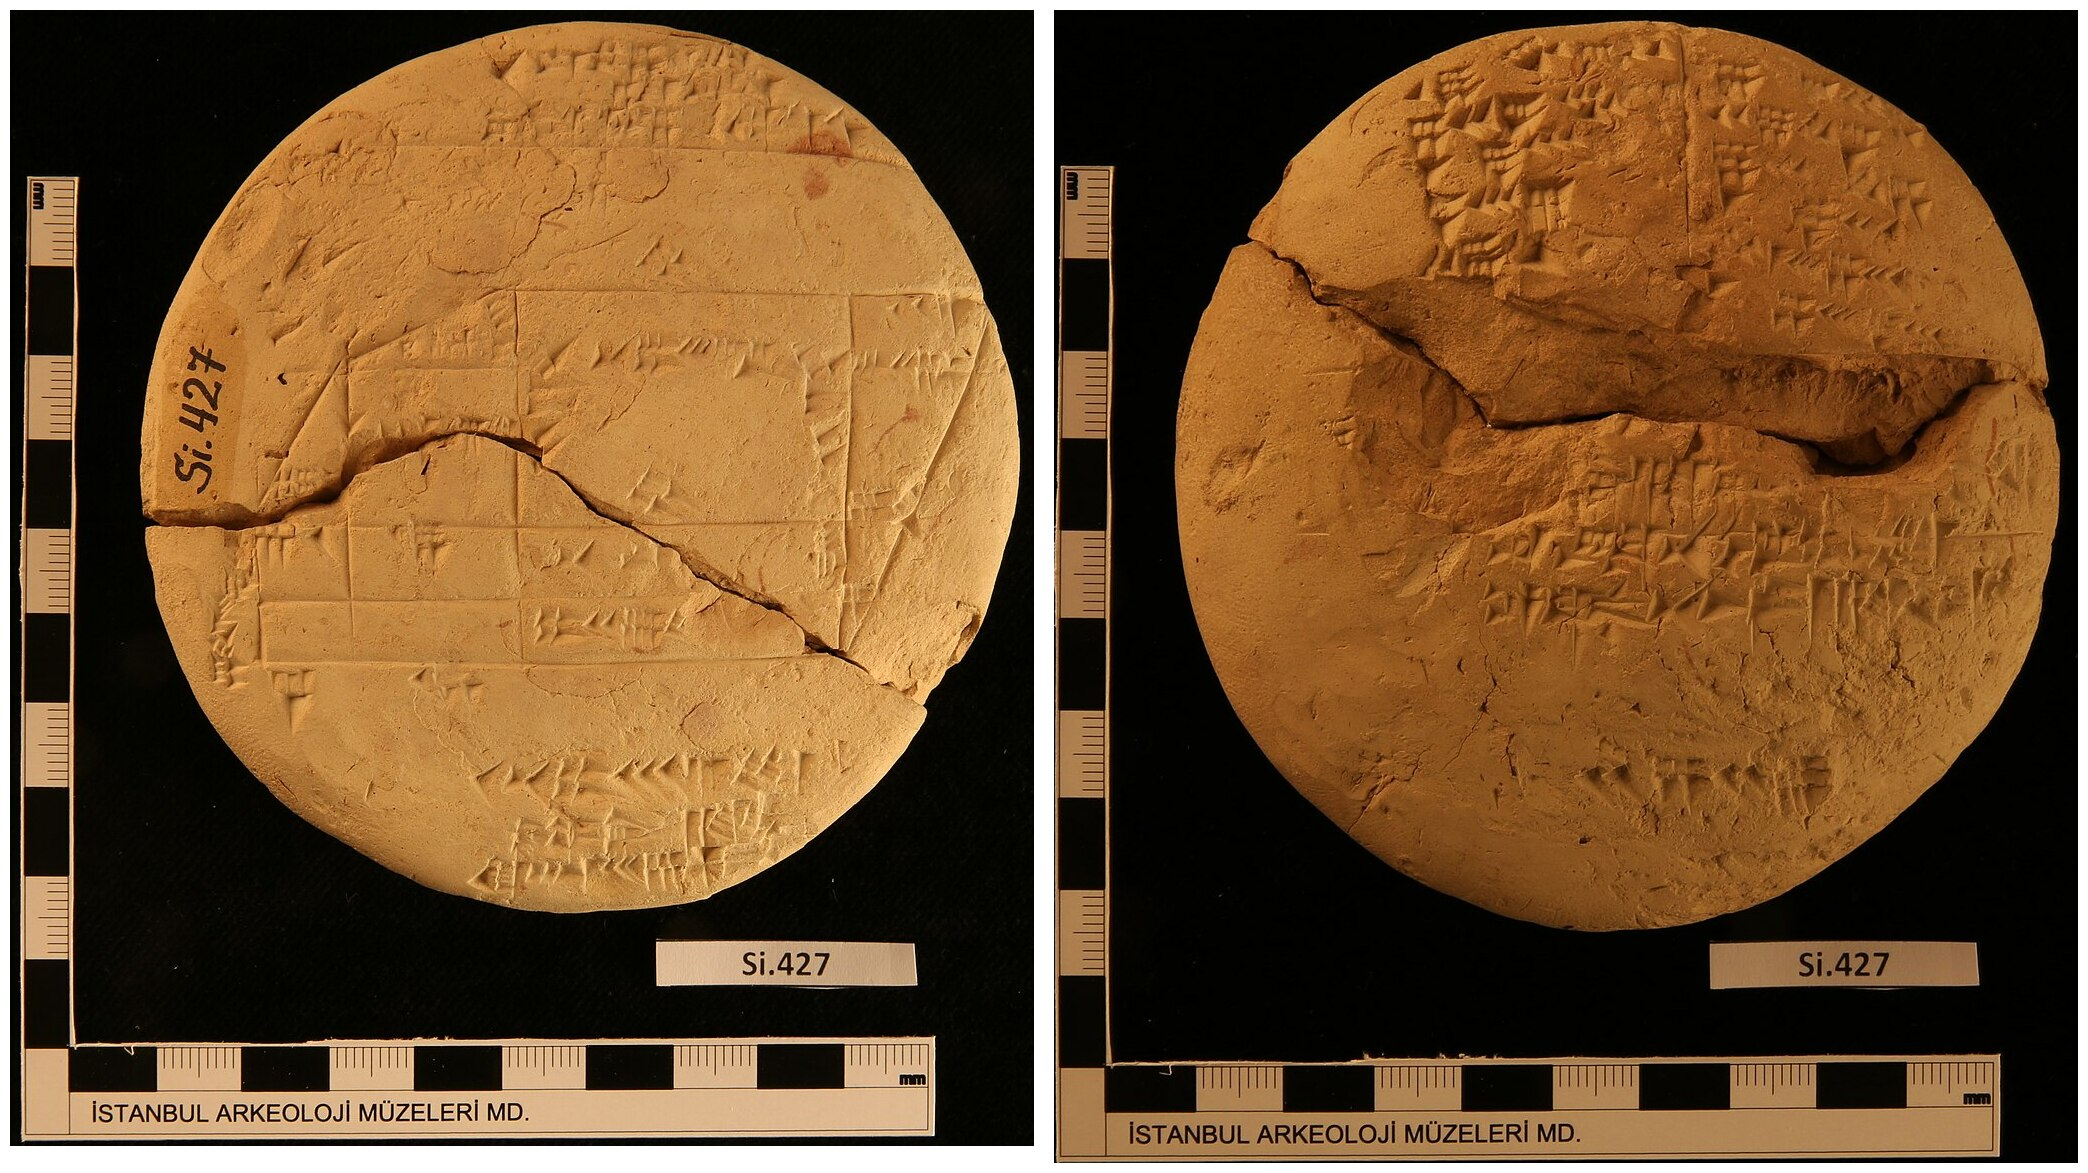
\includegraphics[width=29in]{./figures/si427} 

}

\caption{Photos of the tablet Si. 427 which has recently been identified as the earliest depiction of the Pythagorean theorem [@mansfield2020]. Left: the obverse of the tablet depicts a diagram of a field, inscribed with areas. Right: the reverse of the tablet contains a table of numbers, corresponding to the calculation of the areas. Source: Wikimedia Commons [@mansfield2024].}\label{fig:unnamed-chunk-3}
\end{figure}

For a long time, coordinate systems remained tied to geography and maps. However, with the arrival of the early modern age, this was about to change. In the 16-17th century, the works of the 9th century algebraist Al-Khwarizmi percolated into Europe, and with them the idea of representing unknown quantities by variables (\citeproc{ref-kvasz2006}{Kvasz 2006}). This idea culminated with Descartes, who introduced the concept of visualizing algebraic relationships as objects in a 2D plane, forging a powerful link between Euclidean geometry and algebra (\citeproc{ref-friendly2021}{Friendly and Wainer 2021}). Coordinate systems were thus freed of their connection to geography, and the x- and y-axes could now be used to represent an arbitrary ``space'' spanned by two variables.

Descartes' invention of drawing abstract relationships as objects in a 2D plane was initially only used to plot mathematical functions. However, it would not be long until people realized that observations of the real world could be visualized as well. A true pioneer in this arena was William Playfair, who popularized visualization as a way of presenting socioeconomic data and invented many types of plots still in use today, such as the barplot, lineplot, and pie chart (\citeproc{ref-friendly2021}{Friendly and Wainer 2021}). Further, with the emergence of modern nation states in the 19th century, the collection of data and \emph{statistics} (``things of the state,'' \citeproc{ref-etymonline2024}{Online Etymology Dictionary 2024}) became widespread, leading to a ``golden age'' of statistical graphics (\citeproc{ref-beniger1978}{Beniger and Robyn 1978}; \citeproc{ref-friendly2021}{Friendly and Wainer 2021}; \citeproc{ref-young2011}{Young, Valero-Mora, and Friendly 2011}). This period saw the emergence of other graphical lumnaries, such as Étienne-Jules Marey and Charles Joseph Minard (\citeproc{ref-friendly2021}{Friendly and Wainer 2021}), as well as some ingenious examples of the use of statistical graphics to solve real-world problems, including John Snow's investigation into the London cholera outbreak (\citeproc{ref-freedman1999}{Freedman 1999}; \citeproc{ref-friendly2021}{Friendly and Wainer 2021}) and Florence Nightingale's reporting on the unsanitary treatment of wounded British soldiers during the Crimean War (\citeproc{ref-brasseur2005}{Brasseur 2005}), both of which lead to a great reduction of preventable deaths.

Simultaneously, the field of mathematical statistics was also experiencing significant developments. Building upon the foundation laid by mathematical prodigies such as Jakob Bernoulli, Abraham de Moivre, Pierre Simon Laplace, and Carl Friedrich Gauss, early 19th century pioneers such as Adolph Quetelet and Francis Galton began developing statistical techniques for uncovering hidden trends in the newly unearthed treasure trove of socioeconomic data (\citeproc{ref-fienberg1992}{Fienberg 1992}; \citeproc{ref-freedman1999}{Freedman 1999}). In the late 19th and early 20th century, these initial efforts were greatly advanced by the theoretical work of figures such as Karl Pearson, Ronald A. Fisher, Jerzy Neyman, and Harold Jeffreys, who established statistics as a discipline in its own right and facilitated its dissemination throughout many scientific fields (\citeproc{ref-fienberg1992}{Fienberg 1992}).

As mathematical statistics gained prominence in the early 20th century, data visualization declined. Perceived as less rigorous than ``serious'' statistical analysis, it got relegated to an auxiliary position, ushering in ``dark age'' of statistical graphics (\citeproc{ref-friendly2006}{Friendly 2006}; \citeproc{ref-young2011}{Young, Valero-Mora, and Friendly 2011}). This development may have been partly driven by the early frequentist statisticians' aspiration to establish statistics as a foundation for determining objective truths about the world and society, motivated by personal socio-political goals (see \citeproc{ref-clayton2021}{Clayton 2021}). Be it as it may, while statistical graphics also did get popularized and entered the mainstream during this time, only a few interesting developments took place (\citeproc{ref-friendly2021}{Friendly and Wainer 2021}).

However, beginning in the late 1950's, a series of developments took place which would restore the prominence of data visualization and make it more accessible than ever. Firstly, on the theoretical front, the work of certain academic heavy-weights greatly elevated data visualization and its prestige. Particularly, John Tukey (\citeproc{ref-tukey1962}{1962}; \citeproc{ref-tukey1977}{1977}) fervently championed exploratory data analysis and placed data visualization in its centre. Around the same time, Jacques Bertin published his famous \emph{Sémiologie graphique} (\citeproc{ref-bertin1967}{1967}), which was one of the first works to attempt to lay out a comprehensive system of visual encodings and scales. Secondly, at the more applied level, the development of personal computers (see e.g. \citeproc{ref-abbate1999}{Abbate 1999}) and high-level programming languages such as FORTRAN in 1954 (\citeproc{ref-backus1978}{Backus 1978}), made the process of rendering production-grade figures easier and more accessible than ever before. Combined, these developments fueled a surge in the use and dissemination of data visualizations.

As the millennium drew to a close, several other important developments solidified the foundation of static data visualization. First, William Cleveland made significant contributions to the field, laying out many important principles for scientific data visualization (\citeproc{ref-cleveland1985}{Cleveland 1985}, \citeproc{ref-cleveland1993}{1993}). Of note, his seminal study on the impact of the choice of visual encodings on statistical judgements remains widely cited today (\citeproc{ref-cleveland1984}{Cleveland and McGill 1984}). Similarly, Edward Tufte introduced essential principles for designing effective graphics, coining terms such as \emph{chartjunk} and \emph{data-to-ink ratio} (\citeproc{ref-tufte2001}{Tufte 2001}). Finally, Leland Wilkinson's groundbreaking Grammar of Graphics (\citeproc{ref-wilkinson2012}{2012}) introduced a comprehensive system for designing charts based on simple algebraic rules, influencing nearly every subsequent software package and research endeavor in the field of visualization.

\subsection{Early interactive data visualization: By statisticians for statisticians}\label{early-interactive}

Compared to static data visualization, interactive data visualization is much more of a recent development. Consequently, less has been written about its history, owing to the shorter timeline, as well as the rapid evolution of software in the time since its inception and the proprietary nature of some systems. Nevertheless, the brief history of interactive data visualization is still rather compelling.

Following the boom of static data visualization in the 1950's, interactive data visualization would not be left far behind. It started with tools designed for niche, specialized tasks. For example, Fowlkes (\citeproc{ref-fowlkes1969}{1969}) designed a system which allowed the users to view probability plots under different configurations of parameters and transformations, whereas Kruskal (\citeproc{ref-kruskal1964}{1965}) created a tool for visualizing multidimensional scaling.

\begin{figure}

{\centering 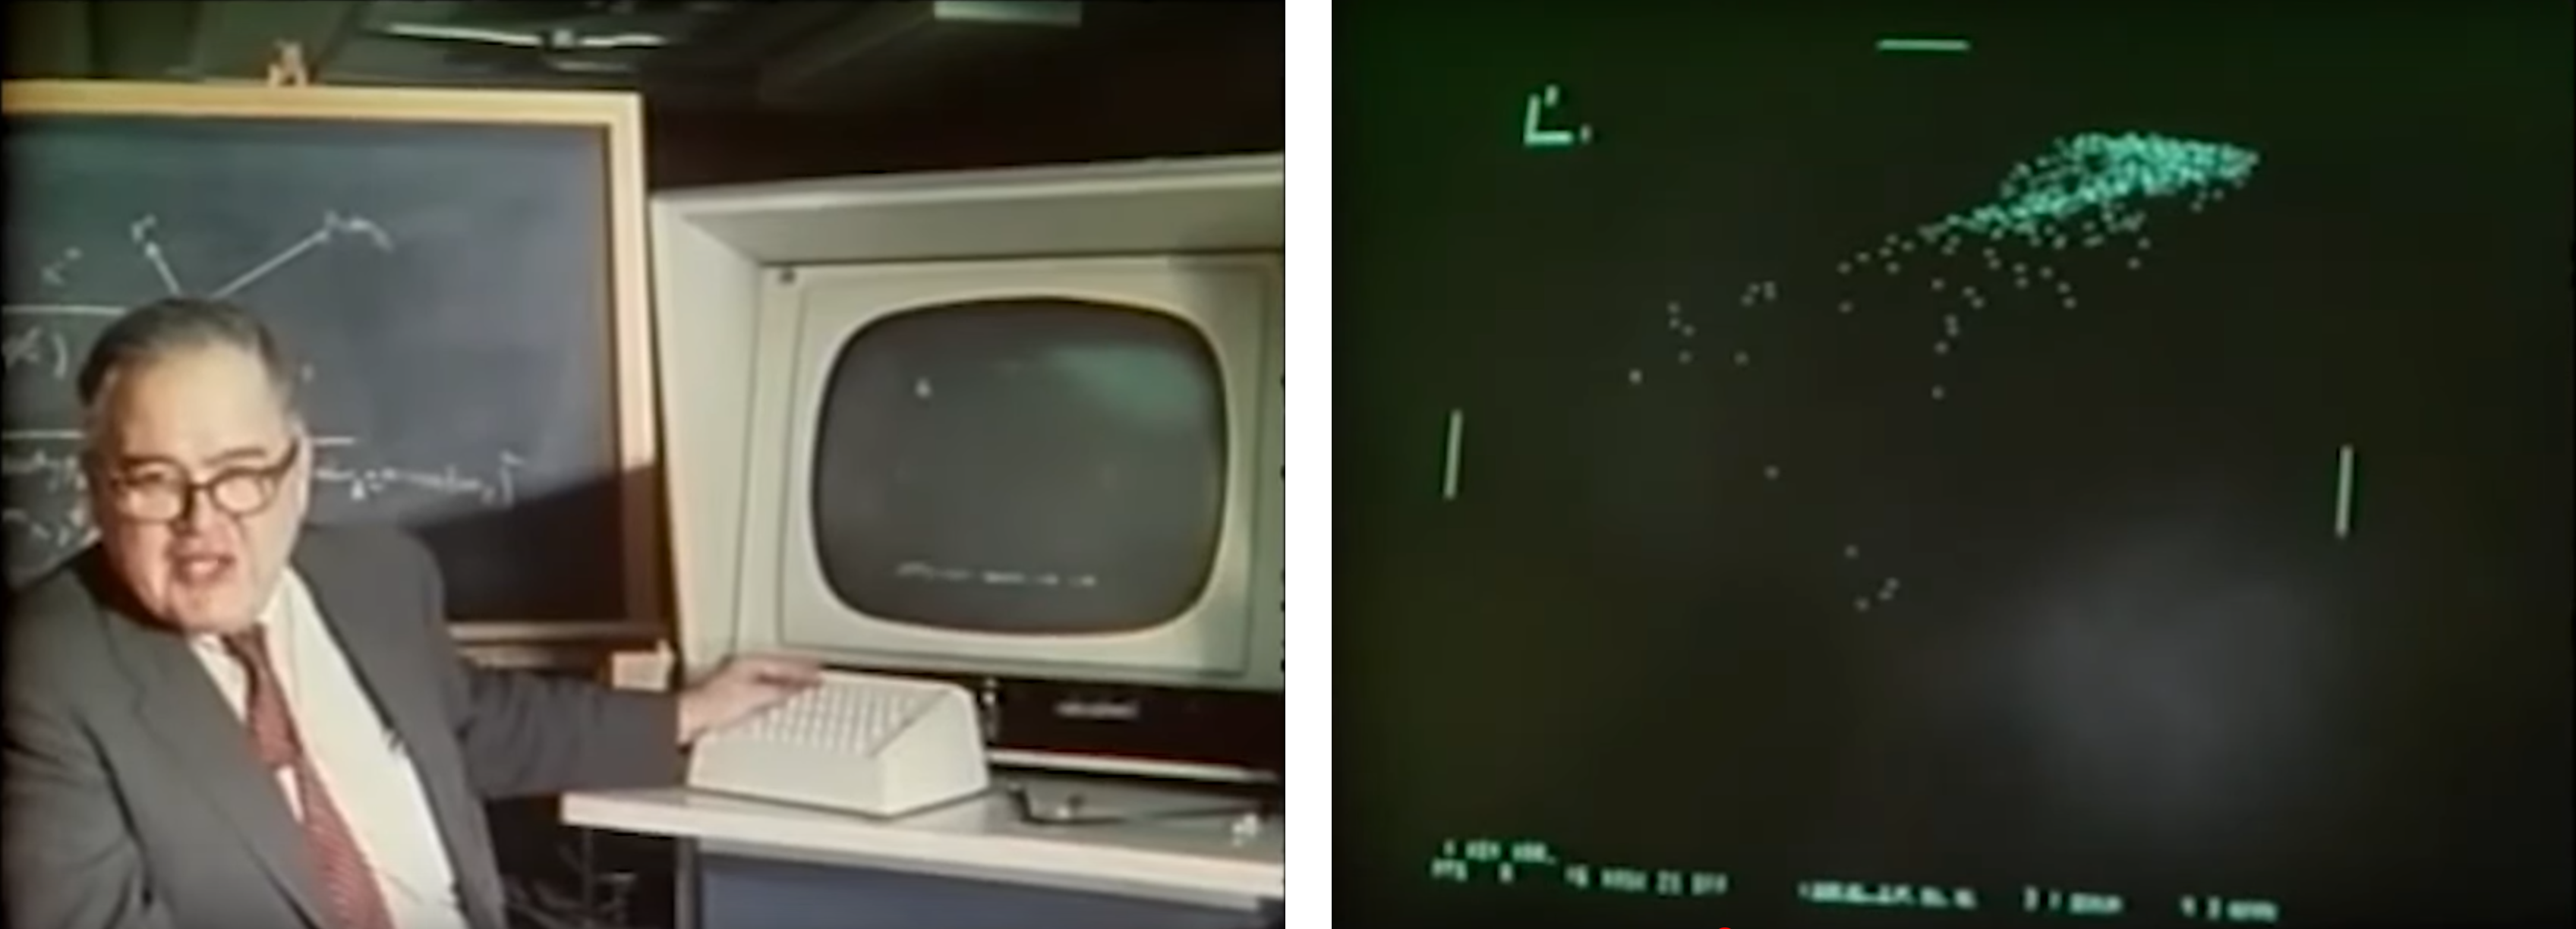
\includegraphics[width=47.12in]{./figures/prim9} 

}

\caption{John Tukey showcasing the PRIM-9 system (left), with an example of a projected scatterplot [right, @fisherkeller1974]. Screenshots were taken from a video available at: [ASA Statistical Graphics Video Library](https://community.amstat.org/jointscsg-section/media/videos))}\label{fig:unnamed-chunk-4}
\end{figure}

However, researchers soon recognized the potential of interactive data visualization as a general-purpose tool for exploring data. The first such general-purpose system was PRIM-9 (\citeproc{ref-fisherkeller1974}{Fisherkeller, Friedman, and Tukey 1974}). PRIM-9 allowed for exploration of multivariate data via interactive features such as projection, rotation, masking, and filtering. Following PRIM-9, the late 1980's saw the emergence of a new generation of systems which provided an even wider range of capabilities. Tools like MacSpin (\citeproc{ref-donoho1988}{Donoho, Donoho, and Gasko 1988}), Data Desk (\citeproc{ref-velleman1989}{Velleman and Paul 1989}), XLISP-STAT (\citeproc{ref-tierney1990}{Tierney 1990}), and XGobi (\citeproc{ref-swayne1998}{Swayne, Cook, and Buja 1998}) introduced features such as interactive scaling, rotation, linked views, and grand tours (for a glimpse into these systems, excellent video-documentaries are available at \href{https://community.amstat.org/jointscsg-section/media/videos}{ASA Statistical Graphics Video Library}).

\begin{figure}

{\centering 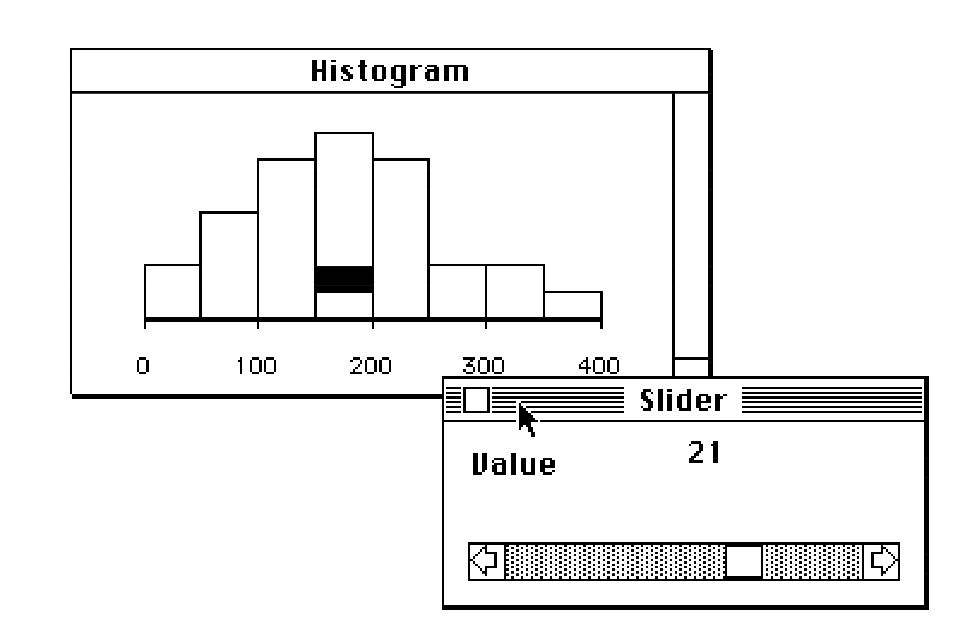
\includegraphics[width=13.29in]{./figures/xlisp-stat} 

}

\caption{Example of interactive control of histogram highlighting in XLISP-STAT. Note that, unlike in many current data visualization systems, aggregation plots were sensitive to data order (not commutative). This non-commutative behavior meant that, for instance, a highlighted segment could appear in the middle of a bar (as seen in the figure above) or multiple non-adjacent highlighted cases might appear as 'stripes'. Figure reproduced from @tierney1990.}\label{fig:xlisp-stat}
\end{figure}

\subsubsection{Open-source Statistical Computing}\label{open-source-statistical-computing}

The proliferation of open-source, general-purpose statistical computing software such as S and R further democratized the access to interactive data visualization tools. Building on XGobi's foundation, GGobi (\citeproc{ref-swayne2003}{Swayne et al. 2003}), expanded upon on XGobi and provided an integration layer for R. Other tools like MANET (\citeproc{ref-unwin1996}{Unwin et al. 1996}) and Mondrian (\citeproc{ref-theus2002}{Theus 2002}) introduced sophisticated linking techniques, with features such as selection sequences, allowing the users to combine a series of selections via logical operators (see also \citeproc{ref-unwin2006}{Unwin et al. 2006}). Further, iPlots (\citeproc{ref-urbanek2003}{Urbanek and Theus 2003}) implemented a general framework for interactive plotting in R, allowing not only for one-shot rendering interactive figures from R but also for direct programmatic manipulation. This package was later expanded expanded for big data capabilities in iPlots eXtreme (\citeproc{ref-urbanek2011}{Urbanek 2011}). Finally, the \texttt{cranvas} package (\citeproc{ref-xie2014}{Xie, Hofmann, and Cheng 2014}) introduced a reactive programming paradigm for defining the infrastructure for interactive graphics directly in R, using the model-view-controller (MVC) architecture.

\begin{figure}

{\centering 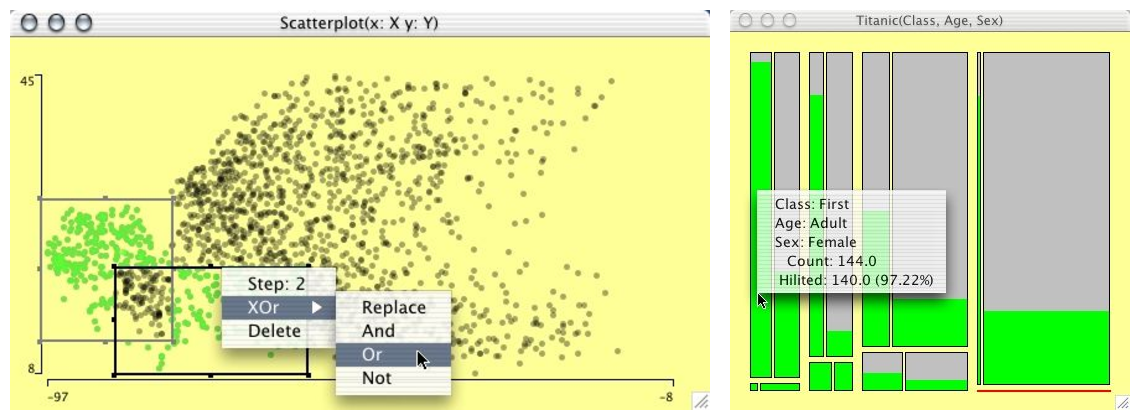
\includegraphics[width=15.83in]{./figures/mondrian} 

}

\caption{Examples of interactive features in Mondrian [@theus2002]: selection operators (left) and mosaic plot with querying (right).}\label{fig:unnamed-chunk-5}
\end{figure}

Alongside the more general interactive data visualization frameworks mentioned above, there were also more specialized packages designed for specific techniques and models. For instance, \texttt{KLIMT} was developed for interactive visualization of classification and regression trees (\citeproc{ref-urbanek2001}{Urbanek and Unwin 2001}; \citeproc{ref-urbanek2002}{Urbanek 2002}). Similarly, packages like \texttt{tourr} (\citeproc{ref-wickham2011}{Wickham 2011}), \texttt{spinifex} (\citeproc{ref-spyrison2020}{Spyrison and Cook 2020}), \texttt{liminal} (\citeproc{ref-lee2021}{Lee 2021}; \citeproc{ref-lee2022a}{Lee, Laa, and Cook 2022}) provided tools for exploring large multivariate data sets via grand tour projections (see \citeproc{ref-cook1995}{Cook et al. 1995}). Generally, over time, there seems to have been a trend towards more of these specialized tools within the R community, and fewer of the general, high-level frameworks (although there were some notable exceptions, such as the \texttt{loon} package, \citeproc{ref-waddell2023}{Waddell and Oldford 2023}). Currently, it seems that R users typically encounter interactive visualizations as part of Shiny (\citeproc{ref-shiny2024}{Chang et al. 2024}) dashboards, or through R wrappers of interactive data visualization packages ported over from the JavaScript ecosystem (see Section \ref{web-based}).

\subsubsection{Common features and limitations of early interactive systems}\label{common-features-and-limitations-of-early-interactive-systems}

A common thread among these interactive data visualization systems is that they were designed by statisticians with primary focus on data exploration. High-level analytic features such as linked views, rotation/projection, and interactive manipulation of model parameters made frequent appearance. While these features were powerful, they also contributed to a steeper learning curve, potentially limiting adoption by users without a strong data analytic background. Furthermore, these early tools were typically standalone applications, with only later packages like GGobi and iplots offering integration with other data analysis software and languages. Finally, they often offerered only limited customization options and this made them less suitable for data presentation.

\subsection{Interactive data visualization and the internet: Web-based interactivity}\label{web-based}

The end of the millennium marked the arrival of a new class of technologies which impacted interactive data visualization just as much as almost every other field of human endeavor. The rise of the internet in the mid 1990's made it possible to create interactive applications that could be accessed by anyone, from anywhere. This was aided by the dissemination of robust and standardized web browsers, as well as the development of JavaScript as a high-level programming language for the web (for a tour of the language's history, see e.g. \citeproc{ref-wirfs-brock2020}{Wirfs-Brock and Eich 2020}). Soon, interactive visualizations became just one of many emerging technologies within the burgeoning web ecosystem.

Early web-based interactive data visualization systems tended to rely on external plugins. Examples of these include Prefuse (\citeproc{ref-heer2005}{Heer, Card, and Landay 2005}) and Flare (developed around 2008, \citeproc{ref-flare2020}{Blokt 2020}), which leveraged the Java runtime and Adobe Flash Player, respectively. However, as browser technologies advanced, particularly as JavaScript's performance improved thanks to advances in just-in-time compilation (JIT, see e.g. \citeproc{ref-clark2017}{Clark 2017}; \citeproc{ref-dao2020}{Dao 2020}), it became possible to create complex interactive experiences directly in the browser. This led to the emergence of several popular web-native interactive data visualization systems in the early 2010s, many of which remain widely used today.

\subsubsection{D3}\label{d3}

D3.js (\citeproc{ref-bostock2022}{Bostock 2022}) is one of the earliest and most influential web-based visualization systems. As a general, low-level framework for visualizing data, D3 provides of a suite of specialized JavaScript modules for various aspects of the data visualization workflow, including data parsing, transformation, scaling, and DOM interaction.

For instance, here's how to create a basic scatterplot in D3:

\begin{Shaded}
\begin{Highlighting}[]
\ImportTok{import} \OperatorTok{*} \ImportTok{as}\NormalTok{ d3 }\ImportTok{from} \StringTok{"d3"}\OperatorTok{;}

\KeywordTok{const}\NormalTok{ plot }\OperatorTok{=} \BuiltInTok{document}\OperatorTok{.}\FunctionTok{querySelector}\OperatorTok{\textless{}}\BuiltInTok{HTMLDivElement}\OperatorTok{\textgreater{}}\NormalTok{(}\StringTok{"\#d3{-}plot"}\NormalTok{)}\OperatorTok{!;}
\KeywordTok{const}\NormalTok{ data }\OperatorTok{=}\NormalTok{ [}
\NormalTok{  \{ }\DataTypeTok{x}\OperatorTok{:} \DecValTok{1}\OperatorTok{,} \DataTypeTok{y}\OperatorTok{:} \FloatTok{0.41}\NormalTok{ \}}\OperatorTok{,}
\NormalTok{  \{ }\DataTypeTok{x}\OperatorTok{:} \DecValTok{2}\OperatorTok{,} \DataTypeTok{y}\OperatorTok{:} \FloatTok{4.62}\NormalTok{ \}}\OperatorTok{,}
\NormalTok{  \{ }\DataTypeTok{x}\OperatorTok{:} \DecValTok{3}\OperatorTok{,} \DataTypeTok{y}\OperatorTok{:} \FloatTok{7.62}\NormalTok{ \}}\OperatorTok{,}
\NormalTok{  \{ }\DataTypeTok{x}\OperatorTok{:} \DecValTok{4}\OperatorTok{,} \DataTypeTok{y}\OperatorTok{:} \FloatTok{6.54}\NormalTok{ \}}\OperatorTok{,}
\NormalTok{  \{ }\DataTypeTok{x}\OperatorTok{:} \DecValTok{5}\OperatorTok{,} \DataTypeTok{y}\OperatorTok{:} \FloatTok{9.61}\NormalTok{ \}}\OperatorTok{,}
\NormalTok{]}\OperatorTok{;}

\KeywordTok{const}\NormalTok{ margin }\OperatorTok{=}\NormalTok{ \{ }\DataTypeTok{top}\OperatorTok{:} \DecValTok{10}\OperatorTok{,} \DataTypeTok{right}\OperatorTok{:} \DecValTok{30}\OperatorTok{,} \DataTypeTok{bottom}\OperatorTok{:} \DecValTok{30}\OperatorTok{,} \DataTypeTok{left}\OperatorTok{:} \DecValTok{60}\NormalTok{ \}}\OperatorTok{;}
\KeywordTok{const}\NormalTok{ width }\OperatorTok{=} \PreprocessorTok{parseFloat}\NormalTok{(plot}\OperatorTok{.}\AttributeTok{style}\OperatorTok{.}\AttributeTok{width}\NormalTok{)}\OperatorTok{;}
\KeywordTok{const}\NormalTok{ height }\OperatorTok{=} \PreprocessorTok{parseFloat}\NormalTok{(plot}\OperatorTok{.}\AttributeTok{style}\OperatorTok{.}\AttributeTok{height}\NormalTok{)}\OperatorTok{;}

\CommentTok{// Create a SVG element, resize it, and append it to \#d3{-}plot}
\KeywordTok{const}\NormalTok{ svg }\OperatorTok{=}\NormalTok{ d3}
  \OperatorTok{.}\FunctionTok{select}\NormalTok{(}\StringTok{"\#d3{-}plot"}\NormalTok{)}
  \OperatorTok{.}\FunctionTok{append}\NormalTok{(}\StringTok{"svg"}\NormalTok{)}
  \OperatorTok{.}\FunctionTok{attr}\NormalTok{(}\StringTok{"width"}\OperatorTok{,}\NormalTok{ width }\OperatorTok{+}\NormalTok{ margin}\OperatorTok{.}\AttributeTok{left} \OperatorTok{+}\NormalTok{ margin}\OperatorTok{.}\AttributeTok{right}\NormalTok{)}
  \OperatorTok{.}\FunctionTok{attr}\NormalTok{(}\StringTok{"height"}\OperatorTok{,}\NormalTok{ height }\OperatorTok{+}\NormalTok{ margin}\OperatorTok{.}\AttributeTok{top} \OperatorTok{+}\NormalTok{ margin}\OperatorTok{.}\AttributeTok{bottom}\NormalTok{)}
  \OperatorTok{.}\FunctionTok{append}\NormalTok{(}\StringTok{"g"}\NormalTok{)}
  \OperatorTok{.}\FunctionTok{attr}\NormalTok{(}\StringTok{"transform"}\OperatorTok{,} \StringTok{"translate("} \OperatorTok{+}\NormalTok{ margin}\OperatorTok{.}\AttributeTok{left} \OperatorTok{+} \StringTok{","} \OperatorTok{+}\NormalTok{ margin}\OperatorTok{.}\AttributeTok{top} \OperatorTok{+} \StringTok{")"}\NormalTok{)}\OperatorTok{;}

\CommentTok{// Create x and y scales and append them to}
\KeywordTok{const}\NormalTok{ scaleX }\OperatorTok{=}\NormalTok{ d3}\OperatorTok{.}\FunctionTok{scaleLinear}\NormalTok{()}\OperatorTok{.}\FunctionTok{domain}\NormalTok{([}\DecValTok{0}\OperatorTok{,} \DecValTok{6}\NormalTok{])}\OperatorTok{.}\FunctionTok{range}\NormalTok{([}\DecValTok{0}\OperatorTok{,}\NormalTok{ width])}\OperatorTok{;}
\KeywordTok{const}\NormalTok{ scaleY }\OperatorTok{=}\NormalTok{ d3}\OperatorTok{.}\FunctionTok{scaleLinear}\NormalTok{()}\OperatorTok{.}\FunctionTok{domain}\NormalTok{([}\DecValTok{10}\OperatorTok{,} \DecValTok{0}\NormalTok{])}\OperatorTok{.}\FunctionTok{range}\NormalTok{([}\DecValTok{0}\OperatorTok{,}\NormalTok{ height])}\OperatorTok{;}
\NormalTok{svg}
  \OperatorTok{.}\FunctionTok{append}\NormalTok{(}\StringTok{"g"}\NormalTok{)}
  \OperatorTok{.}\FunctionTok{attr}\NormalTok{(}\StringTok{"transform"}\OperatorTok{,} \StringTok{"translate(0,"} \OperatorTok{+}\NormalTok{ height }\OperatorTok{+} \StringTok{")"}\NormalTok{)}
  \OperatorTok{.}\FunctionTok{call}\NormalTok{(d3}\OperatorTok{.}\FunctionTok{axisBottom}\NormalTok{(scaleX))}\OperatorTok{;}
\NormalTok{svg}\OperatorTok{.}\FunctionTok{append}\NormalTok{(}\StringTok{"g"}\NormalTok{)}\OperatorTok{.}\FunctionTok{call}\NormalTok{(d3}\OperatorTok{.}\FunctionTok{axisLeft}\NormalTok{(scaleY))}\OperatorTok{;}

\CommentTok{// Add points}
\NormalTok{svg}
  \OperatorTok{.}\FunctionTok{append}\NormalTok{(}\StringTok{"g"}\NormalTok{)}
  \OperatorTok{.}\FunctionTok{selectAll}\NormalTok{(}\StringTok{"dot"}\NormalTok{)}
  \OperatorTok{.}\FunctionTok{data}\NormalTok{(data)}
  \OperatorTok{.}\FunctionTok{enter}\NormalTok{()}
  \OperatorTok{.}\FunctionTok{append}\NormalTok{(}\StringTok{"circle"}\NormalTok{)}
  \OperatorTok{.}\FunctionTok{attr}\NormalTok{(}\StringTok{"cx"}\OperatorTok{,}\NormalTok{ (d) }\KeywordTok{=\textgreater{}} \FunctionTok{scaleX}\NormalTok{(d}\OperatorTok{.}\AttributeTok{x}\NormalTok{))}
  \OperatorTok{.}\FunctionTok{attr}\NormalTok{(}\StringTok{"cy"}\OperatorTok{,}\NormalTok{ (d) }\KeywordTok{=\textgreater{}} \FunctionTok{scaleY}\NormalTok{(d}\OperatorTok{.}\AttributeTok{y}\NormalTok{))}
  \OperatorTok{.}\FunctionTok{attr}\NormalTok{(}\StringTok{"r"}\OperatorTok{,} \DecValTok{2}\NormalTok{)}\OperatorTok{;}
\end{Highlighting}
\end{Shaded}

\begin{figure}

{\centering 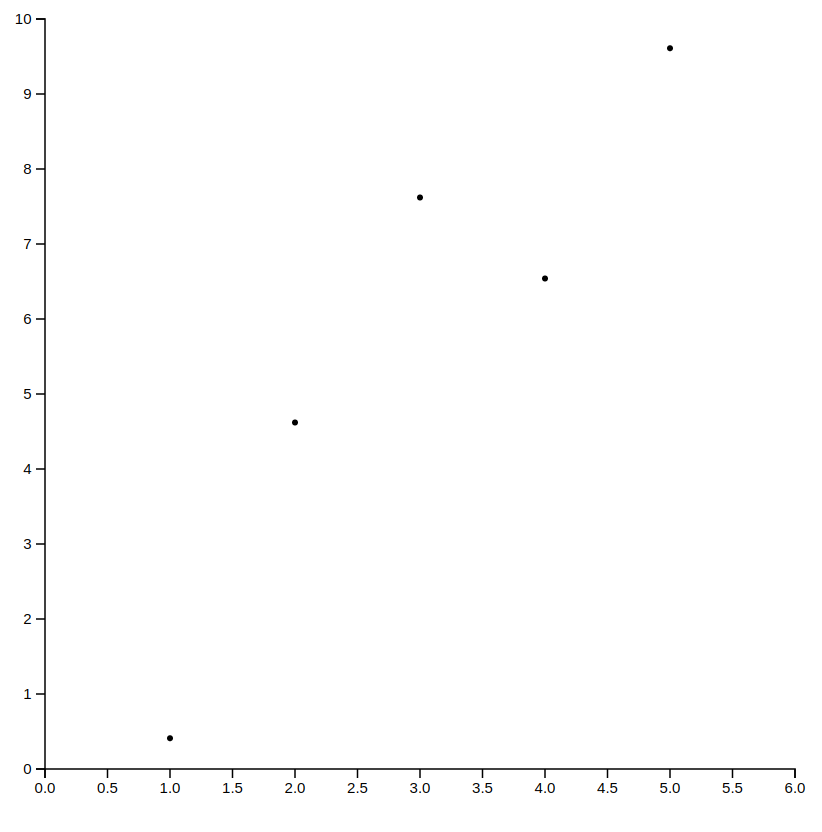
\includegraphics[width=11.42in]{./figures/d3-scatterplot} 

}

\caption{Example of a scatterplot in D3.js. The code was taken from D3 Graph Gallery [@holtz2022b] and adjusted to use ES6 syntax and slightly more informative variable names/comments.}\label{fig:d3-scatterplot}
\end{figure}

As you can see from Figure \ref{fig:d3-scatterplot} and the corresponding code, D3 is a fairly low-level framework. Compared to typical high-level plotting functionalities such as those provided by base R or \texttt{ggplot2} (\citeproc{ref-r2024}{R Core Team 2024}; \citeproc{ref-wickham2016}{Wickham 2016}), the user has to handle many low-level details such as scaling and appending of primitives explicitly. This is also the case with interaction. While D3 does provide some methods for handling reactive DOM events, it does not itself provide a system for dispatching and coordinating these events - instead, it delegates this responsibility to the user, and encourages the use of reactive Web frameworks such as React (\citeproc{ref-react2024}{Meta 2024}), Vue (\citeproc{ref-vue2024}{Evan You and the Vue Core Team 2024}), or Svelte (\citeproc{ref-svelte2024}{Rich Harris and the Svelte Core Team 2024}).

Finally, D3.js visualizations are rendered as Scalable Vector Graphics (SVG) by default. This ensures lossless scaling but may impact rendering performance at high data volumes. While various unofficial alternative rendering engines based on the HTML 5 Canvas element or WebGL, do exist, there are no official libraries with such functionalities as of this date.

\subsubsection{Plotly and Highcharts}\label{plotly-and-highcharts}

Building upon the low-level infrastructure that D3 provides, many packages such as Plotly.js (\citeproc{ref-plotly2022}{Plotly Inc. 2022}) and Highcharts (\citeproc{ref-highcharts2024}{Highsoft 2024}) provide high-level abstractions which make the process of building interactive figures easier for the average user. Unlike D3 which provides low-level utilities such as data transformations, scales, and geometric objects, these packages provide a simple declarative framework for rendering entire plots using a static {[}JSON{]} schema.

Here's how to render the same scatterplot in Plotly:

\begin{Shaded}
\begin{Highlighting}[]
\KeywordTok{const}\NormalTok{ data }\OperatorTok{=}\NormalTok{ [\{}
  \DataTypeTok{x}\OperatorTok{:}\NormalTok{ [}\DecValTok{1}\OperatorTok{,} \DecValTok{2}\OperatorTok{,} \DecValTok{3}\OperatorTok{,} \DecValTok{4}\OperatorTok{,} \DecValTok{5}\OperatorTok{,} \DecValTok{6}\NormalTok{]}\OperatorTok{,}
  \DataTypeTok{y}\OperatorTok{:}\NormalTok{ [}\FloatTok{0.41}\OperatorTok{,} \FloatTok{4.62}\OperatorTok{,} \FloatTok{7.62}\OperatorTok{,} \FloatTok{6.54}\OperatorTok{,} \FloatTok{9.61}\NormalTok{]}\OperatorTok{,}
  \DataTypeTok{mode}\OperatorTok{:} \StringTok{\textquotesingle{}markers\textquotesingle{}}\OperatorTok{,}
  \DataTypeTok{type}\OperatorTok{:} \StringTok{\textquotesingle{}scatter\textquotesingle{}}
\NormalTok{\}]}\OperatorTok{;}

\NormalTok{Plotly}\OperatorTok{.}\FunctionTok{newPlot}\NormalTok{(}\StringTok{\textquotesingle{}app\textquotesingle{}}\OperatorTok{,}\NormalTok{ data)}\OperatorTok{;}
\end{Highlighting}
\end{Shaded}

\phantomsection\label{app}

\begin{figure}

{\centering 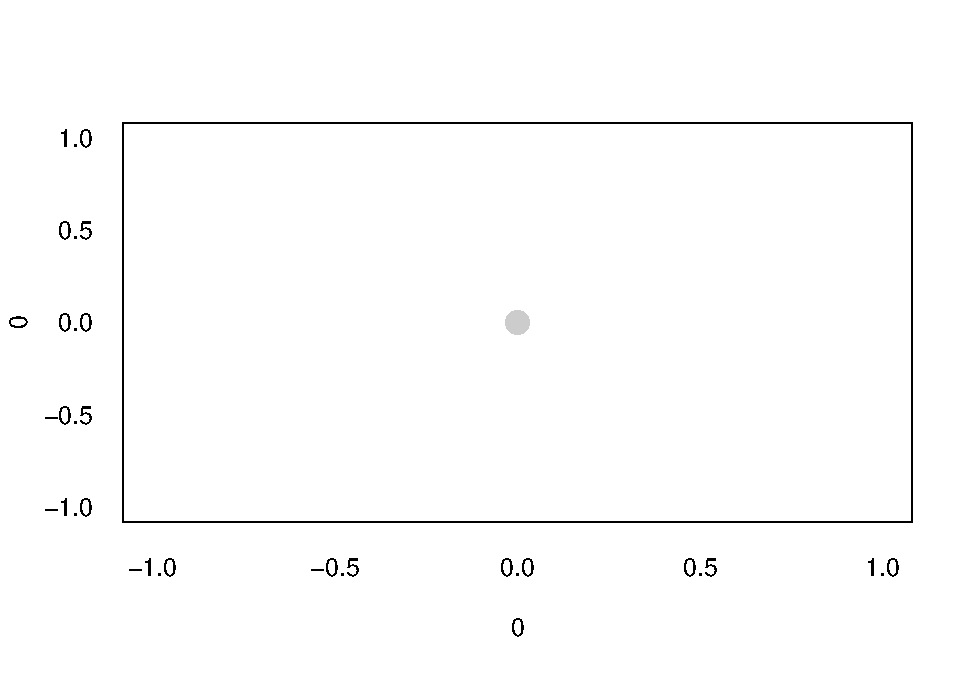
\includegraphics[width=0px,height=0px]{_main_files/figure-latex/plotly-scatterplot-1} 

}

\caption{Example of a scatterplot in Plotly.js. The code was taken from the official Plotly documentation [@plotly2024c] and slightly simplified.}\label{fig:plotly-scatterplot}
\end{figure}

Clearly, compared with the D3 code used to create Figure \ref{fig:d3-scatterplot}, the code for creating Figure \ref{fig:plotly-scatterplot} is much terser. Many details, such as the axis limits and margins, point size and colour, gridlines, and widgets, are handled implicitly, via default values and automatic inference. Also, note that the figure provides some interactive features by default, such as zooming, panning, and tooltip on hover. Reactivity is handled automatically using systems built on the native DOM Event Target interface (\citeproc{ref-mdn2024a}{MDN 2024}).

Highcharts provides a similar JSON-based interface for specifying plots. While perhaps slightly more flexible than Plotly, it also requires more verbose specifications. Because of the similarity, I will not provide a separate example here (interested reader should look up the library website, \citeproc{ref-highcharts2024}{Highsoft 2024}).

Finally, like D3, both plotly.js and Highcharts also render the graphics in SVG by default. However, unlike D3, they both also provide alternative rendering engines based on WebGL (\citeproc{ref-highschartsboost2022}{Highsoft 2022}; \citeproc{ref-plotly2024b}{Plotly Inc. 2024}). This makes them more ergonomic for use with large data sets.

\subsubsection{Vega and Vega-Lite}\label{vega-and-vega-lite}

Vega (\citeproc{ref-satyanarayan2015}{Satyanarayan et al. 2015}; \citeproc{ref-vega2024a}{Vega Project 2024d}) is another popular interactive data visualization package. Like Plotly and Highcharts, Vega is also partially built upon the foundation of D3 and uses JSON schema for plot specification. However, Vega is more low-level and implements a lot of custom functionality. This allows it to offer more fine-grained customization of graphics and interactive behavior, leading to greater flexibility.

However, this added flexibility does come at a cost. Compared to the high-level frameworks like Plotly and Highcharts, Vega is significantly more verbose. For instance, creating a scatterplot matrix with linked selection in Vega requires over 300 lines of JSON specification, not including the data and using default formatting (\citeproc{ref-vega2024b}{Vega Project 2024b}).

Vega-Lite (\citeproc{ref-satyanarayan2015}{Satyanarayan et al. 2015}) attempts to remedy this complexity by providing a high-level interface to Vega. Here's how we can define a scatterplot with zooming, panning, and tooltip on hover in Vega-Lite:

\phantomsection\label{vegalite-plot}

\begin{Shaded}
\begin{Highlighting}[]
\KeywordTok{const}\NormalTok{ spec }\OperatorTok{=}\NormalTok{ \{}
  \DataTypeTok{$schema}\OperatorTok{:} \StringTok{"https://vega.github.io/schema/vega{-}lite/v5.json"}\OperatorTok{,}
  \DataTypeTok{width}\OperatorTok{:} \DecValTok{500}\OperatorTok{,}
  \DataTypeTok{height}\OperatorTok{:} \DecValTok{500}\OperatorTok{,}
  \DataTypeTok{data}\OperatorTok{:}\NormalTok{ \{ }\DataTypeTok{values}\OperatorTok{:}\NormalTok{ [}
\NormalTok{    \{ }\DataTypeTok{x}\OperatorTok{:} \DecValTok{1}\OperatorTok{,} \DataTypeTok{y}\OperatorTok{:} \FloatTok{0.41}\NormalTok{ \}}\OperatorTok{,}
\NormalTok{    \{ }\DataTypeTok{x}\OperatorTok{:} \DecValTok{2}\OperatorTok{,} \DataTypeTok{y}\OperatorTok{:} \FloatTok{4.62}\NormalTok{ \}}\OperatorTok{,}
\NormalTok{    \{ }\DataTypeTok{x}\OperatorTok{:} \DecValTok{3}\OperatorTok{,} \DataTypeTok{y}\OperatorTok{:} \FloatTok{7.62}\NormalTok{ \}}\OperatorTok{,}
\NormalTok{    \{ }\DataTypeTok{x}\OperatorTok{:} \DecValTok{4}\OperatorTok{,} \DataTypeTok{y}\OperatorTok{:} \FloatTok{6.54}\NormalTok{ \}}\OperatorTok{,}
\NormalTok{    \{ }\DataTypeTok{x}\OperatorTok{:} \DecValTok{5}\OperatorTok{,} \DataTypeTok{y}\OperatorTok{:} \FloatTok{9.61}\NormalTok{ \}]}
\NormalTok{  \}}\OperatorTok{,}
  \DataTypeTok{mark}\OperatorTok{:}\NormalTok{ \{}\StringTok{"type"}\OperatorTok{:} \StringTok{"point"}\OperatorTok{,} \StringTok{"tooltip"}\OperatorTok{:} \KeywordTok{true}\NormalTok{\}}\OperatorTok{,}
  \DataTypeTok{encoding}\OperatorTok{:}\NormalTok{ \{}
    \DataTypeTok{x}\OperatorTok{:}\NormalTok{ \{ }\DataTypeTok{field}\OperatorTok{:} \StringTok{"x"}\OperatorTok{,} \DataTypeTok{type}\OperatorTok{:} \StringTok{"quantitative"}\NormalTok{ \}}\OperatorTok{,}
    \DataTypeTok{y}\OperatorTok{:}\NormalTok{ \{ }\DataTypeTok{field}\OperatorTok{:} \StringTok{"y"}\OperatorTok{,} \DataTypeTok{type}\OperatorTok{:} \StringTok{"quantitative"}\NormalTok{ \}}
\NormalTok{  \}}\OperatorTok{,}
  \DataTypeTok{params}\OperatorTok{:}\NormalTok{ [\{ }\DataTypeTok{name}\OperatorTok{:} \StringTok{"grid"}\OperatorTok{,} \DataTypeTok{select}\OperatorTok{:} \StringTok{"interval"}\OperatorTok{,} \DataTypeTok{bind}\OperatorTok{:} \StringTok{"scales"}\NormalTok{ \}]}
\NormalTok{\}}\OperatorTok{;}

\FunctionTok{vegaEmbed}\NormalTok{(}\StringTok{"\#vegalite{-}plot"}\OperatorTok{,}\NormalTok{ spec)}\OperatorTok{;}
\end{Highlighting}
\end{Shaded}

Note that the zooming and panning capability is provided by the \texttt{params} property, which declaratively specifies a list of plot parameters that can be modified by interaction (see \citeproc{ref-vegalite2024a}{Vega Project 2024c}). In the case above, the specification creates a two-way binding between plot scales and mouse selection events (\citeproc{ref-vegalite2024b}{Vega Project 2024a}).

\subsubsection{Common features and limitations of web-based interactive systems}\label{common-features-and-limitations-of-web-based-interactive-systems}

In general, these contemporary web-based interactive data visualization systems offer a great deal of flexibility, making them well-suited to modern data presentation. However, all of this expressiveness does seem to come at a cost. Compared to the earlier statistical graphics systems, described in Section \ref{early-interactive}, many of the more advanced features that used to be common are either missing or require a significant effort to implement, such that they are only accessible to expert users. This is evidenced by their infrequent appearance in documentation and example gallery pages.

For instance, the \href{https://r-graph-gallery.com/interactive-charts.html}{R Graph Gallery entry on Interactive Charts} (\citeproc{ref-holtz2022}{Holtz 2022}) features multiple interactive figures implemented in the JavaScript libraries described above. However, all of these examples show only surface-level, single-plot interactive features such zooming, panning, hovering, 3D rotation, and node repositioning. The \href{https://dash.plotly.com/interactive-graphing}{Plotly Dash documentation page on Interactive Visualizations} (\citeproc{ref-plotly2022}{Plotly Inc. 2022}) does feature two examples of simple linked cross-filtering, however, the vast majority of visualizations in the \href{https://plotly.com/r/}{Plotly R Open Source Graphing Library documentation page} (\citeproc{ref-plotly2022}{Plotly Inc. 2022}) show examples only surface-level interactivity. Similarly, \href{https://vega.github.io/vega-lite/examples/\#interactive-charts}{VegaLite Gallery pages on Interactive Charts} (\citeproc{ref-vegalite2022}{Vega Project 2022}) feature many examples, however, only a limited number of examples show linked or parametric interactivity (see e.g.~\href{https://vega.github.io/vega-lite/examples/\#interactive-multi-view-displays}{Interactive Multiview Displays}). Finally, the \href{https://jkunst.com/highcharter/articles/showcase.html}{Highcharter Showcase Page} (\citeproc{ref-kunst2022}{Kunst 2022}) does not feature any examples of linking.

Even when advanced features such as linking and parametric manipulation are supported, they are often limited in some way. For example, the following is a quote from the website of Crosstalk, a package designed to enable linking in R, using web-based interactive widgets created with the \texttt{htmlwidgets} package (\citeproc{ref-htmlwidgets2021}{Vaidyanathan et al. 2021}) or R Shiny (\citeproc{ref-shiny2024}{Chang et al. 2024}):

\begin{quote}
``Crosstalk currently only works for linked brushing and filtering of views that show individual data points, not aggregate or summary views (where ``observations'' is defined as a single row in a data frame). For example, histograms are not supported since each bar represents multiple data points; but scatter plot points each represent a single data point, so they are supported.''

\begin{itemize}
\tightlist
\item
  Posit (formerly RStudio Inc.) (\citeproc{ref-crosstalk2025}{2025})
\end{itemize}
\end{quote}

Of course, with enough effort, these web-based visualization systems can still be used to create rich figures with advanced interactive features such as linked views and parametric interaction. However, implementing these features often requires stepping down a level of abstraction and dealing with low-level language primitives. This defeats the purpose of using a high-level libraries and creates a barrier to entry for casual users (\citeproc{ref-keller2024}{Keller, Manz, and Gehlenborg 2024}). It also may explain why interactive visualizations are nowadays mainly used for data presentation, not data exploration (\citeproc{ref-batch2017}{Batch and Elmqvist 2017}). With the high upfront cost of learning these package's APIs, creating rich interactive figures may be a task best suited for dedicated developers working inside large organizations, rather than individual researchers/analysts.

\section{What even is interactive data visualization?}\label{what-is-interactive-visualization}

\begin{quote}
If it looks like a duck, swims like a duck, and quacks like a duck, then it probably is a duck.

{[}\ldots{]} The irony is that while the phrase is often cited as proof of abductive reasoning, it is not proof, as the mechanical duck is still not a living duck

\href{https://en.wikipedia.org/wiki/Duck_test}{Duck Test} entry, (\citeproc{ref-wikipedia2022}{Wikipedia 2022})
\end{quote}

In the previous section (Section \ref{brief-history}), I provided an overview of the history and present state of interactive data visualization, discussing a number of features and systems. However, while doing so, I avoided one crucial question: what constitutes an interactive data visualization?

Surprisingly, despite the widespread popularity of interactive visualizations, there is no universally agreed-upon definition of interactivity (\citeproc{ref-vanderplas2020}{Vanderplas, Cook, and Hofmann 2020}). Within the data visualization literature, the terms ``interactive'' and ``interaction'' are rarely explicitly defined. And even when they are, the definitions are often incongruent or even contradictory (see e.g. \citeproc{ref-dimara2019}{Dimara and Perin 2019}; \citeproc{ref-elmqvist2011}{Elmqvist et al. 2011}; \citeproc{ref-pike2009}{Pike et al. 2009}). Finally, similar conceptual ambiguity extends to other terms commonly used in the field, such as a ``dashboard'' (\citeproc{ref-sarikaya2018}{Sarikaya et al. 2018}).

This lack of a clear consensus makes the task of discussing interactive data visualization difficult. Ignoring the issue could lead to confusion, while a truly comprehensive dive into the terminology surrounding interactive data visualization could become excessively verbose, as evidenced by the existence of research papers dedicated to the topic (see e.g. \citeproc{ref-dimara2019}{Dimara and Perin 2019}; \citeproc{ref-elmqvist2011}{Elmqvist et al. 2011}). To address this issue, this section aims to provide a concise overview of how interactivity has been conceptualized in the literature. The goal is to establish a clear framework for understanding ``interactive'' and ``interaction'' within the context of this thesis.

\subsection{Interactive vs.~interacting with}\label{interactive-interacting}

First, the word ``visualization'' in ``interactive data visualization'' can be interpreted in two different ways:

\begin{enumerate}
\def\labelenumi{\arabic{enumi}.}
\tightlist
\item
  As a noun: a concrete chart or figure
\item
  As a nominalized verb: the process of interacting with a figure
\end{enumerate}

In data visualization literature, both interpretations are frequently used, leading to significant ambiguity (\citeproc{ref-dimara2019}{Dimara and Perin 2019}; \citeproc{ref-pike2009}{Pike et al. 2009}; see also \citeproc{ref-yi2007}{Yi et al. 2007}). On one hand, some researchers focus on the mathematical and computational aspects of visualization, discussing specific systems and implementations (see e.g. \citeproc{ref-buja1996}{Buja, Cook, and Swayne 1996}; \citeproc{ref-kelleher2015}{Kelleher and Levkowitz 2015}; \citeproc{ref-leman2013}{Leman et al. 2013}; \citeproc{ref-wills2008}{G. Wills 2008}). Others prioritize the more cognitive or human-computer interaction (HCI) aspects of interactive data visualization, exploring what impact different kinds of visualization techniques have on the user's ability to derive insights from the data (see e.g. \citeproc{ref-brehmer2013}{Brehmer and Munzner 2013}; \citeproc{ref-dimara2019}{Dimara and Perin 2019}; \citeproc{ref-dix1998}{Dix and Ellis 1998}; \citeproc{ref-pike2009}{Pike et al. 2009}; \citeproc{ref-quadri2021}{Quadri and Rosen 2021}; \citeproc{ref-yi2007}{Yi et al. 2007}).

Of course, many interactive data visualization papers discuss both implementation and user experience. However, the dual interpretation of the term ``interactive data visualization'' does complicate literature search. It also highlights the interdisciplinary nature of the field, showing its connections to statistics, computer science, applied mathematics, business analytics, HCI, and cognitive psychology (see \citeproc{ref-brehmer2013}{Brehmer and Munzner 2013}; \citeproc{ref-dimara2019}{Dimara and Perin 2019}). While this interdisciplinary nature of interactive data visualization is certainly a strength, it can also lead to confusion. As such I think it is necessary to clearly define key terms.

To ensure clarity throughout thesis, the term \emph{``interactive data visualization''} will primarily refer to concrete charts or figures. When referring to the \emph{practice} of interactive data visualization, I will attempt to use more active phrasing such as \emph{``interacting with a visualization''} or \emph{``user's interaction with a visualization''}, to indicate that what is being referred to is the activity or process of visualization, rather than any concrete figure or chart.

\subsection{\texorpdfstring{Interactive \emph{enough}?}{Interactive enough?}}\label{interactive-enough}

Even when we use the term ``interactive data visualization'' to refer to concrete charts or figures, the meaning still remains fairly ambiguous. What is the bar for calling a figure ``interactive''? What features should interactive figures have? Surprisingly, it is hard to find consensus on these topics among data visualization researchers, and the criteria tend to vary a lot, such that the same figure may be considered interactive by some but not by others.

Some researchers adopt a broad definition of interactive data visualization, considering almost any figure combined with an interactive graphical user interface (GUI) as interactive, as long as it allows for some level of user manipulation (\citeproc{ref-brodbeck2009}{Brodbeck, Mazza, and Lalanne 2009}). For others, the speed of the computer's responses to user input is important, with faster updates translating to greater interactivity (\citeproc{ref-becker1987}{Becker and Cleveland 1987}; \citeproc{ref-buja1996}{Buja, Cook, and Swayne 1996}). Some also differentiate between ``interactive'' and ``dynamic'' manipulation, such that interactive manipulation involves discrete actions such as pressing a button or selecting an item from a drop-down menu, whereas dynamic manipulation involves continuous actions, like moving a slider or clicking-and-dragging to highlight a rectangular area (\citeproc{ref-rheingans2002}{Rheingans 2002}; \citeproc{ref-jankun2007}{Jankun-Kelly, Ma, and Gertz 2007}; see also \citeproc{ref-dimara2019}{Dimara and Perin 2019}).

However, many other researchers ascribe to a much narrower view of interactive data visualization, which hinges on high-level analytic features that allow efficient exploration of the data. These features include the ability to generate different views of the data (by e.g.~zooming, panning, sorting, and filtering), and the reactive propagation of changes between connected or ``linked'' parts of a figure (\citeproc{ref-kehrer2012}{Kehrer et al. 2012}; \citeproc{ref-buja1996}{Buja, Cook, and Swayne 1996}; \citeproc{ref-keim2002}{Keim 2002}; \citeproc{ref-unwin1999}{Unwin 1999}; \citeproc{ref-chen2008}{Chen et al. 2008}). An often cited guideline is the visual information seeking mantra: overview first, zoom and filter, then details-on-demand (\citeproc{ref-shneiderman2003}{Shneiderman 2003}). Similarly, in visual analytics research, a distinction is made between ``surface-level'' (or ``low-level'') and ``parametric'' (or ``high-level'') interactions, where surface-level interactions manipulate attributes of the visual domain only (e.g.~zooming and panning), whereas parametric interactions manipulate attributes of mathematical models or algorithms underlying the visualization (\citeproc{ref-leman2013}{Leman et al. 2013}; \citeproc{ref-self2018}{Self et al. 2018}; \citeproc{ref-pike2009}{Pike et al. 2009}).

Table \ref{tab:definitions} provides a concise summary of the several perspectives on interactivity discussed above. It meant to serve as a reference point for future discussions within the text, though it is important to note that this is not an exhaustive list. For a more comprehensive taxonomy of interactive visualization systems and features, see e.g. Dimara and Perin (\citeproc{ref-dimara2019}{2019}), Yi et al. (\citeproc{ref-yi2007}{2007}).

\begin{table}
\centering
\caption{\label{tab:definitions}Summary of the perspectives on interactivity}
\centering
\begin{tabular}[t]{l|l|l}
\hline
Name & Details & Selected references\\
\hline
User interaction & The user can interactively manipulate the figure in some way & @brodbeck2009\\
\hline
Real-time updates & The user's interactions propagate into the visualization with little to no lag & @becker1987, @buja1996, @jankun2007, and @rheingans2002\\
\hline
Plot- and data-space manipulation & The user can interactively explore different parts of the data set by doing actions which effectively amount to "subsetting" rows of the data (e.g. zooming, panning, and filtering) & @buja1996, @keim2002, @shneiderman2003, and @unwin1999\\
\hline
Linked views & The user's interactions propagate across multiple plots (e.g. linked highlighting) & @buja1996, @keim2002, @kehrer2012, @unwin1999, @theus2008, @wilhelm2008, @wills2008\\
\hline
Parametric updates & The user can manipulate the parameters of some underlying mathematical model or algorithm (e.g. histogram bins, grand tour projections, etc...) & @leman2013, @pike2009\\
\hline
\end{tabular}
\end{table}

\subsection{Complexity of interactive features}\label{complexity-of-features}

The way we define interactivity is not just a matter of taste or preference: it has a significant impact on the complexity and feasibility of our systems. As we will see in Section \ref{common-features}, some simple features are fairly easy to implement, requiring just a thin interactive layer over a static data visualization system, whereas others come with a significant overhead, requiring an entirely different framework than static visualization.

To make the point with a particularly blunt example, many programming languages support a read-evaluate-print loop (REPL). This allows interactive code execution from the command line: the user inputs code, the interpreter evaluates it, outputs results, and waits for more input. If the language supports plotting, running code to generate plots could be considered an ``interactive data visualization system.'' User interaction with the REPL modifies the visual output, and with fast-enough input, updates could appear almost instantly (thus satisfying the user interaction and real-time update definitions of interactivity, see table). This would make almost every programming language an ``interactive data visualization system'', requiring no additional effort.

However, I would argue that, today, this view stretches the concept of interactivity. It is true that, historically, the command line was considered a highly interactive user interface (see e.g. \citeproc{ref-foley1990}{Foley 1990}; \citeproc{ref-howard1995}{Howard and MacEachren 1995}). However, with advancements in processor speeds and the widespread adoption of graphical user interfaces (GUIs), user expectations have evolved. Nowadays, we typically associate interactivity with direct manipulation of visual elements and immediate feedback (\citeproc{ref-dimara2019}{Dimara and Perin 2019}; \citeproc{ref-urbanek2011}{Urbanek 2011}). Thus, we can see that what's considered ``interactive'' evolves over time.

But even with figures that are manipulated directly, there still are considerable differences in what different features imply for implementation requirements. Some features, like changing color or opacity of points in a scatterplot affect only the visual attributes of the plot and not the underlying data representation. This makes them simple to implement as they do not require any specialized data structures or complex computations, and the primary cost lies in re-rendering the visualization.

In contrast, some interactive features require a lot more infrastructure. For instance, filtering, linked highlighting, or parametric interaction require specialized data structures and algorithms beyond those that would be required in static plots. This is because, each time the user engages in an interaction, entirely new summaries of the underlying data may need to be computed.

To give a concrete example, when a user selects several points in a linked scatterplot (see Section \ref{linked-selection}), we first have to find the ids of all the selected cases, recompute the statistics underlying all other linked plots (such as counts/sums in barplots or histograms), train all of the relevant scales, and only then can we re-render the figure. Likewise, when interactively manipulating a histogram's binwidth, we need to recompute the number of cases in each bin whenever the binwidth changes. To maintain the illusion of smooth, ``continuous'' interaction (\citeproc{ref-dimara2019}{Dimara and Perin 2019}), these computations need to happen fast, and as such, computational efficiency becomes imperative at high data volumes.

\subsection{Working definition}\label{working-definition}

As discussed in previous sections, the definition ``interactive data visualization'' varies across fields and researchers. Moreover, when building interactive data visualization systems, different definitions imply varying levels of implementation complexity. Thus, we need to establish clear criteria for our specific definition.

Data visualization can be broadly categorized into two primary modes: presentation and exploration. While both modes share a bulk of common techniques, each comes with a different set of goals and challenges (\citeproc{ref-kosara2016}{Kosara 2016}). Data presentation starts from the assumption that we have derived most of the important insights from our data already, and the goal is now to communicate these insights clearly and make an impactful and lasting impression (\citeproc{ref-kosara2016}{Kosara 2016}). In contrast, data exploration begins from a position of incomplete knowledge - we accept that there are facts about our data we might not be aware of. Thus, when we explore data with visualizations, the goal is to help us see what we might otherwise miss or might not even think to look for (\citeproc{ref-tukey1977}{Tukey et al. 1977}; \citeproc{ref-unwin2018}{Unwin 2018}).

However, it is not always the case that more complex visuals necessarily translate to better statistical insights. In static visualization, it is a well-established that plots can include seemingly sophisticated features which do not promote the acquisition of statistical insights in any way (\citeproc{ref-cairo2014}{Cairo 2014}, \citeproc{ref-cairo2019}{2019}; \citeproc{ref-gelman2013}{Gelman and Unwin 2013}; \citeproc{ref-tufte2001}{Tufte 2001}). Similarly, adding interactivity to a visualization does not always improve its statistical legibility (see e.g. \citeproc{ref-abukhodair2013}{Abukhodair et al. 2013}; \citeproc{ref-franconeri2021}{Franconeri et al. 2021}).

I propose to treat interactive features the same way we treat visual features in static visualization. Specifically, I propose the following working definition:

\begin{quote}
When building interactive data visualization systems, we should prioritize interactive features which promote statistical understanding.
\end{quote}

If we accept this proposition, then several important consequences follow. First, we must favor high-level, data-dependent, parametric interactions over the purely graphical ones. That is not to say that purely graphical interactive features cannot useful. For instance, in the case of overplotting, changing the size or alpha of points in a scatterplot can help us see features that would otherwise remain hidden. Nevertheless, I argue that the ability to see entirely new representations of the data is what makes some interactive data visualizations systems particularly powerful. The interactive features that enable this, such as linked highlighting and parameter manipulation, go beyond aesthetics, and empower the users to explore the data in a much more dynamic way, compared to static graphics.

\subsection{Common interactive features}\label{common-features}

This section describes several common types of interactive features that tend to frequently appear in general interactive data visualization systems. It is only meant as an overview (for more comprehensive taxonomies of interactive features, see \citeproc{ref-dimara2019}{Dimara and Perin 2019}; \citeproc{ref-unwin2006}{Unwin et al. 2006}; \citeproc{ref-yi2007}{Yi et al. 2007}). For each feature, I highlight its core properties, common use cases, and implementation requirements.

\subsubsection{Changing size and opacity}\label{changing-size-and-opacity}

One of the simplest and most widely-implemented interactive features is the ability to adjust the size and opacity of geometric objects. This feature gives the user the ability to dynamically shrink or grow objects and make semi-transparent, fully transparent, or opaque.

The ability to shrink objects or make them semi-transparent can be particularly useful at high data volumes, since this can reveal trends that may be otherwise hidden due to overplotting. For example, in scatterplots, shrinking points and making them semi-transparent makes it possible to identify high-density regions and can in fact provide an approximation to a 2D kernel density plot (see e.g. \citeproc{ref-dang2010}{Dang, Wilkinson, and Anand 2010}). The same applies to all other types of plots where the where objects or glyphs may be plotted on top of each other at high densities, such as parallel coordinate plots (\citeproc{ref-theus2008}{Theus 2008}).

This feature usually fairly easy to implement, since it involves manipulating visual attributes only. Specifically, in many interactive systems, size and alpha multipliers are independent parameters of the visual representation, which do not depend on the underlying data in any way. In other words, when we manipulate size or opacity of geometric objects in our plots, we do not need to worry about what data these objects represent. Compared to other interactive features, this makes it relatively simple to add this functionality to an existing static visualization system (see \citeproc{ref-bracsoveanu2017}{Braşoveanu et al. 2017}).

\subsubsection{Zooming and panning}\label{zooming-and-panning}

Another two significantly related interactive features are zooming and panning. They are often used in tandem, and both involve interactive manipulation of scale limits. For this reason, I discuss them here simultaneously, in a single subsection.

Zooming, depicted in Figure \ref{fig:zooming}, allows the user to magnify into a specific region of a plot. A common approach involves creating a rectangular selection and the axis scales are then automatically adjusted to match this region, however, other techniques do exist, for instance a symmetric zoom centered on a point using a mouse wheel. Zooming is useful because it allows the user to get a better sense of the trend within the magnified region, and discover patterns that may be otherwise obscured due to overplotting or improper aspect ratio (see e.g. \citeproc{ref-buja1996}{Buja, Cook, and Swayne 1996}; \citeproc{ref-dix1998}{Dix and Ellis 1998}; \citeproc{ref-unwin1999}{Unwin 1999}; \citeproc{ref-theus2008}{Theus 2008}; \citeproc{ref-yi2007}{Yi et al. 2007}).

\begin{figure}

{\centering 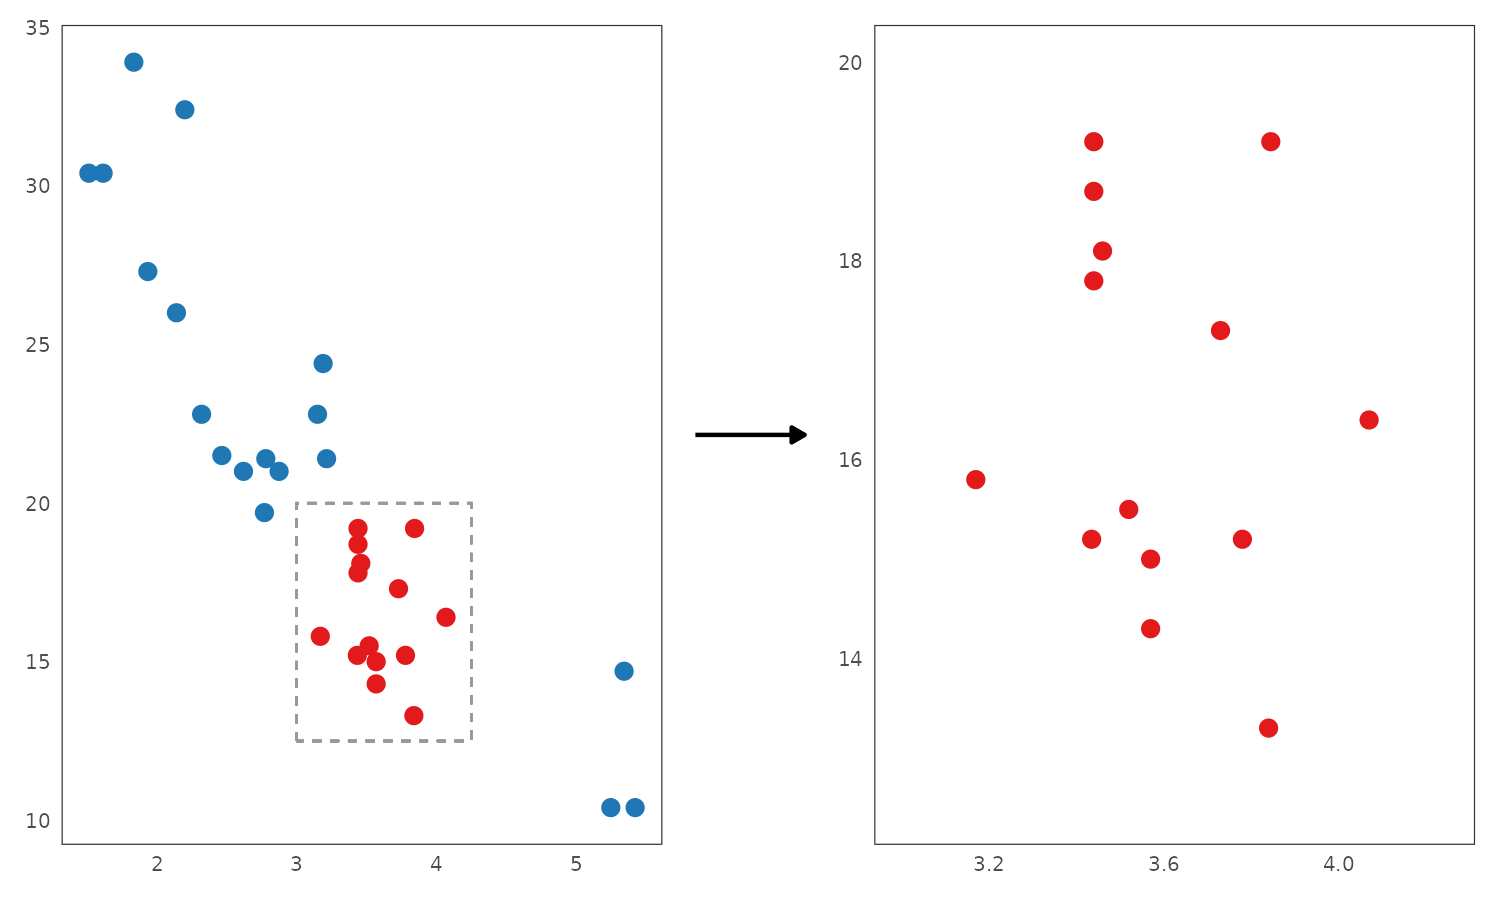
\includegraphics[width=20.83in]{./figures/zooming} 

}

\caption{Zooming involves shrinking the axis limits to obtain a more detailed view of the data. Typically, the user selects a rectangular region of the plot (left) and the plot scales are then adjusted so that the region fills up the entire plot area (right). Notice the change in the axis limits.}\label{fig:zooming}
\end{figure}

After zooming, it is useful to retain the ability to navigate the wider plot region while preserving the current zoom level and aspect ratio. Panning addresses this need. By performing some action, typically right-click and drag, the user can move the center of the zoomed-in region around, exploring different areas of the plot.

\begin{figure}

{\centering 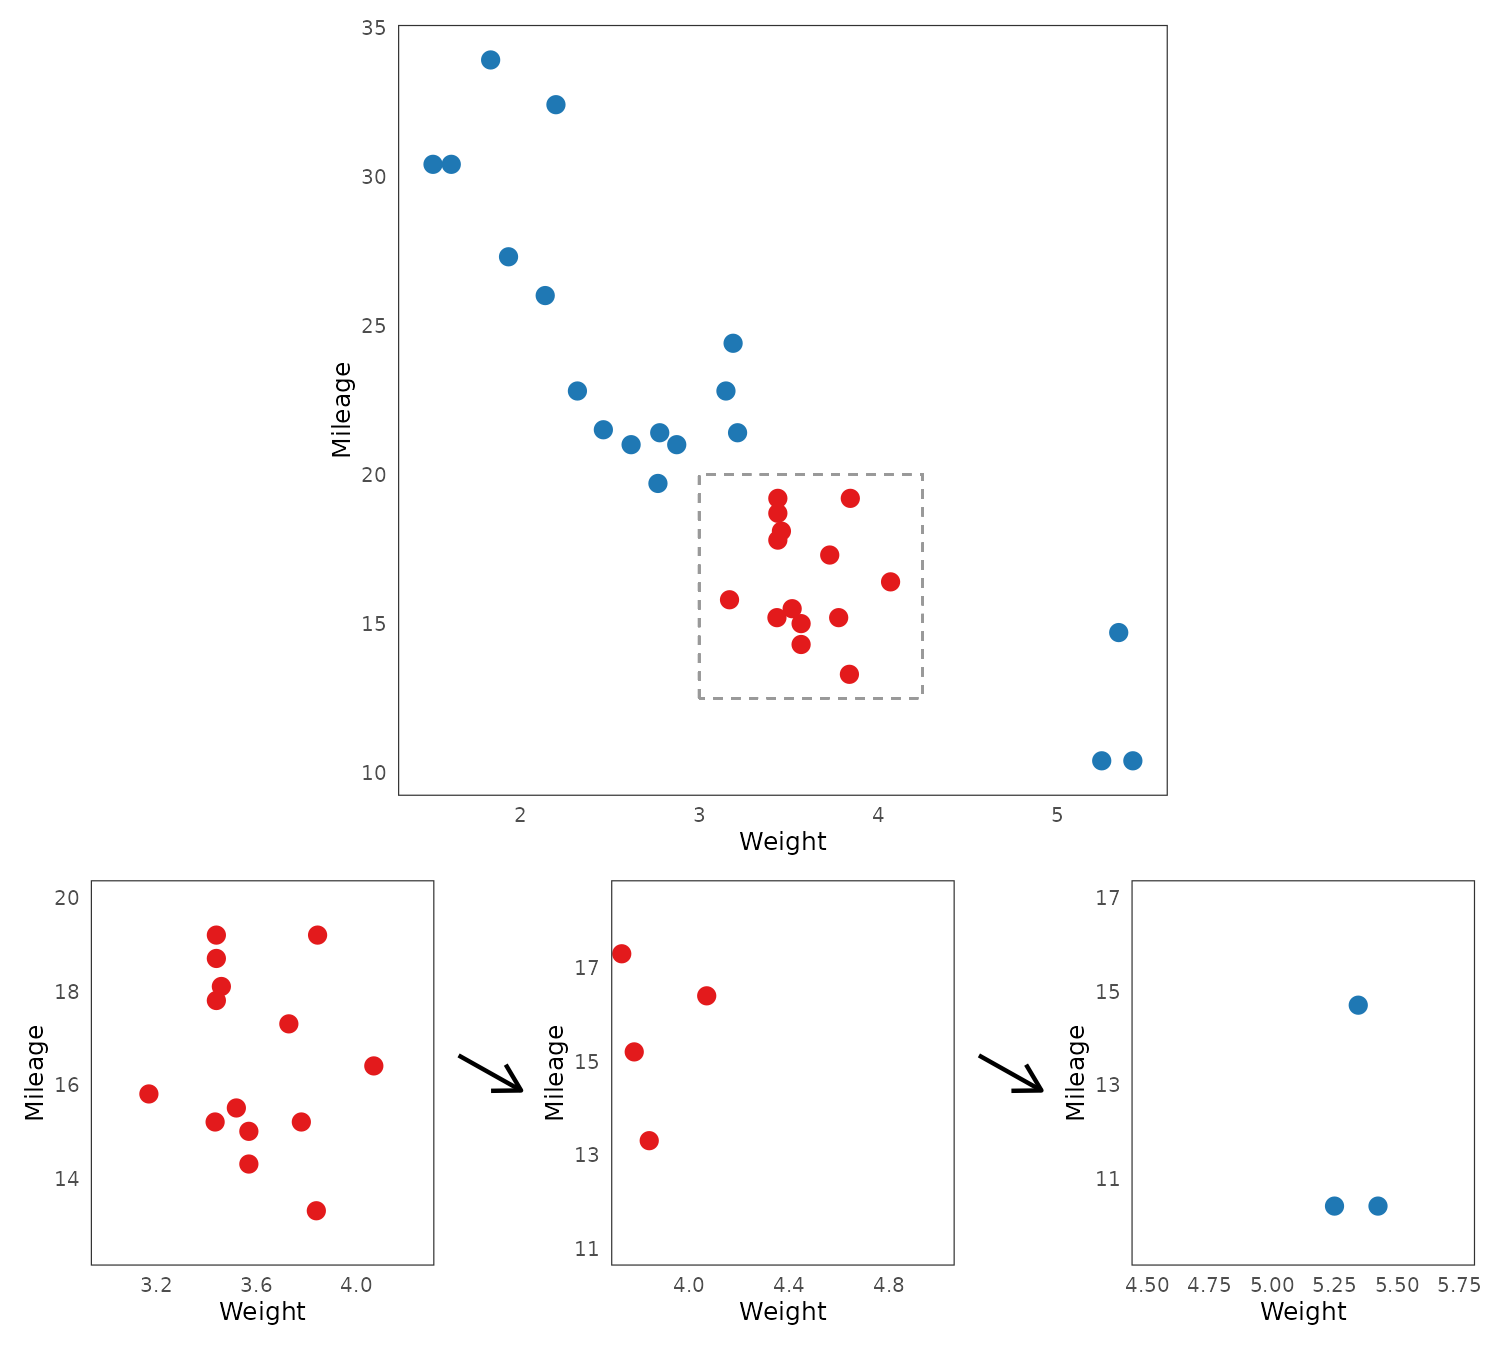
\includegraphics[width=20.83in]{./figures/panning} 

}

\caption{Panning involves moving the axis limits while retaining the same zoom level and axis ratio. After zooming into a rectangular region (top row), the user can around the plot region, usually by clicking and dragging (bottom row).}\label{fig:panning}
\end{figure}

Zooming and panning can be implemented by manipulating scales only, and this also makes them generally fairly straightforward to implement, similar to changing size and opacity. However, there are a few issues to consider. First, whereas continuous axes can be be zoomed and/or panned by simply modifying the axis limits, zooming discrete axes requires a bit more nuance (see e.g. \citeproc{ref-wilkinson2012}{Wilkinson 2012}). Second, it is often desirable to give the user the ability to zoom-in multiple levels deep, and this makes maintaining a reversible history of previous zoom-states essential (\citeproc{ref-unwin1999}{Unwin 1999}). Third, at times, it can be useful to link scale updates across multiple plots, such that, for example, zooming or panning a plot in a scatterplot matrix produces the same actions in other plots with the same variable on one of the axes. Finally, an advanced feature that can be also quite useful is semantic or logical zooming (\citeproc{ref-keim2002}{Keim 2002}; \citeproc{ref-unwin1999}{Unwin 1999}; \citeproc{ref-yi2007}{Yi et al. 2007}). This technique goes beyond magnifying objects; it also increases the level of detail the objects display as the user zooms in. Semantic zooming can be particularly powerful when combined with hierarchical data such as geographic information, however, it also introduces additional complexity, since the effects of the zoom action propagate beyond x- and y-axis scales.

\subsubsection{Querying}\label{querying}

Querying is another popular interactive feature that is usually fairly straightforward to implement. As shown in Figure \ref{fig:querying}, the way querying is typically implemented is that when a user mouses over a particular geometric object, a small table of key-value pairs is displayed via a tool-tip/pop-up, showing a summary of the underlying data point(s) (\citeproc{ref-urbanek2003}{Urbanek and Theus 2003}; \citeproc{ref-xie2014}{Xie, Hofmann, and Cheng 2014}). This makes it possible to look up precise values that would otherwise be available only approximately via the visual representation.

\begin{figure}

{\centering 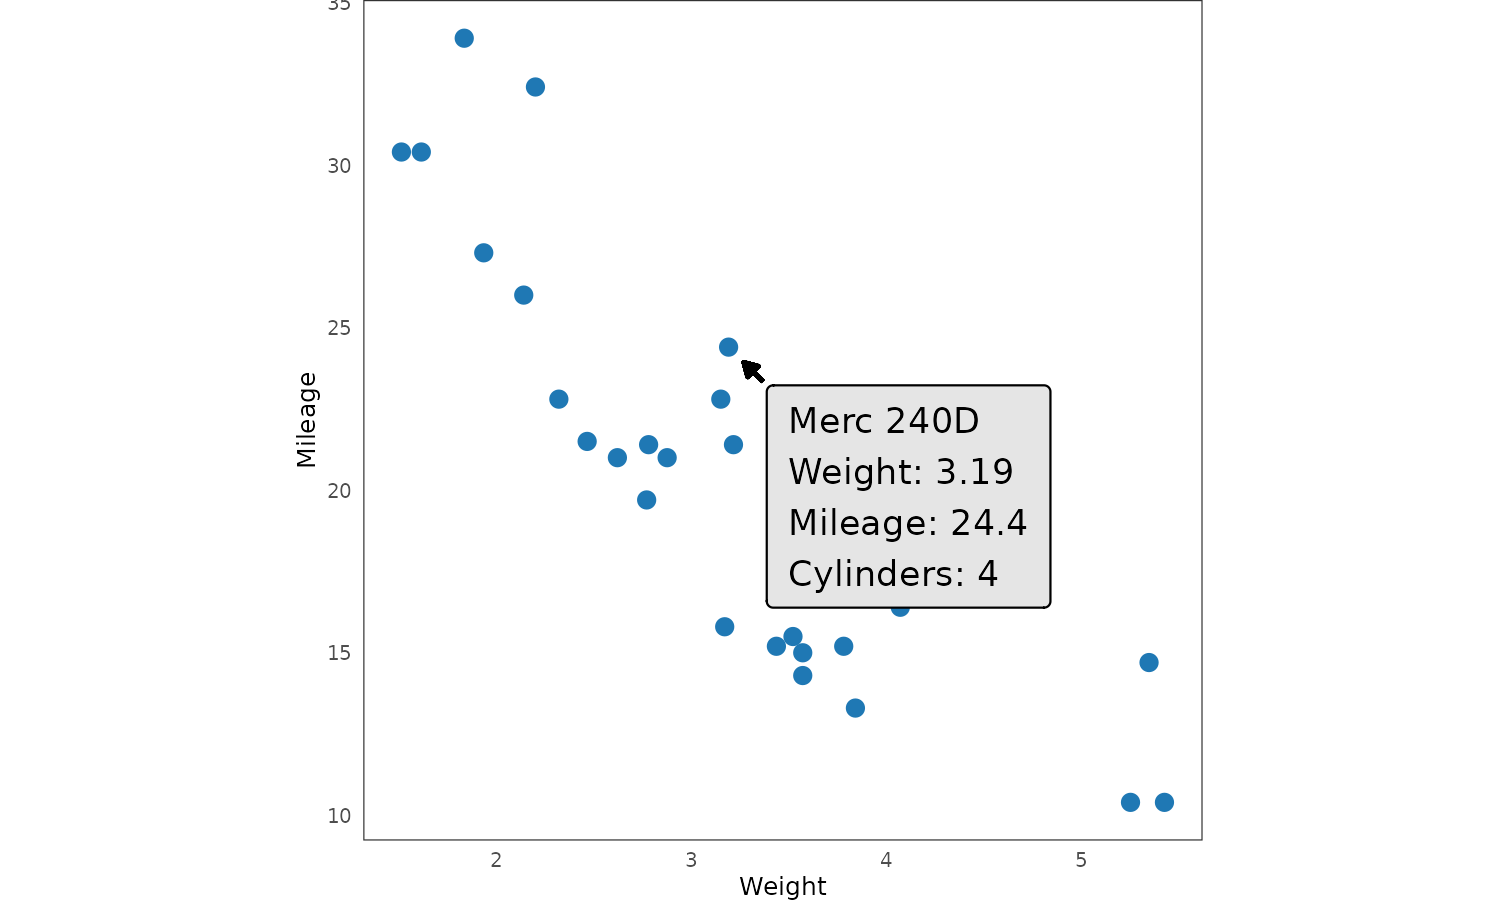
\includegraphics[width=20.83in]{./figures/querying} 

}

\caption{Querying involves hovering over an object to display its associated data values in a table or pop-up. Notice that this can include both plotted values (`weight`, `mileage`) as well as values that are not directly represented in the plot (car name, `cylinders`).}\label{fig:querying}
\end{figure}

Querying is useful because it combines the best features of graphics and tables. Specifically, it allows the user to overcome Tukey's famous prescriptions: ``graphics are for the qualitative/descriptive {[}\ldots{]} never for the carefully quantitative (tables do that better)'', and: ``graphics are for comparison {[}\ldots{]} not for access to individual amounts'' (\citeproc{ref-tukey1993}{Tukey 1993}). By providing the option to query individual objects, the user can seamlessly transition between the high-level analytic overview of the graphic and low-level quantitative detail of a table. This facilitates high-precision analytic tasks, such as identifying specific outliers or calculating exact magnitudes of differences (\citeproc{ref-unwin2006}{Unwin et al. 2006}).

Additionally, querying also allow us to show more information than is displayed via the visual encodings alone (see again Figure \ref{fig:querying}). Specifically, whereas most plots can encode only two or three variables, we can assign an arbitrary number of key-value pairs to the rows of the query table/pop-up. However, it is crucial to balance the level of detail against visual clutter. Too many rows may overtax the attention of the user and also can lead to clipping/overplotting issues, if the query table cannot fit inside the plotting area. Further, there are \hyperref[bidirectional-communication]{better methods} for retrieving very detailed information from interactive visualizations.

Finally, while querying is also one of the more straightforward features, its implementation does present certain challenges. First, a naive implementation might simply display derived data values in the state just before they are mapped to visual attributes via scales, however, these are not always the most informative. For instance, in a stacked barplot, returning the original (unstacked) values is more useful than the stacked ones. Second, aggregate plots such as barplots or histograms do generally present some design decisions (see \citeproc{ref-unwin2006}{Unwin et al. 2006}). In the case of one-to-one plots such as scatterplots, query data for an object (point) can be obtained by simply retrieving the corresponding row. However, in aggregate plots like barplots and histograms, a single object may correspond to multiple rows. This necessitates summarizing the underlying data, and often there may be no single ``correct'' summary. For instance, when querying a bar in a barplot, should we return the sum of the underlying continuous variable, some other numeric summary such as the mean or maximum, the set of all unique values, multiple of these summaries, or perhaps something else entirely? Similar ambiguities arise when querying objects which are partially selected or highlighted (see Section \ref{linked-selection}): should the query return summaries corresponding to the entire object, the highlighted parts, or both?

\subsubsection{Sorting and reordering}\label{sorting-and-reordering}

With plots of discrete (unordered) data, a highly useful feature can be to sort or reorder objects based on some criterion (see \citeproc{ref-unwin2000}{Unwin 2000}; \citeproc{ref-unwin2006}{Unwin et al. 2006}). For example, with barplots, in the absence of other ordering rules, bars are typically ordered by the lexographical order of the x-axis variable. However, sometimes, we can glean interesting patterns by sorting the bars in some other order, for example by their height, see Figure \ref{fig:sorting}.

\begin{figure}

{\centering 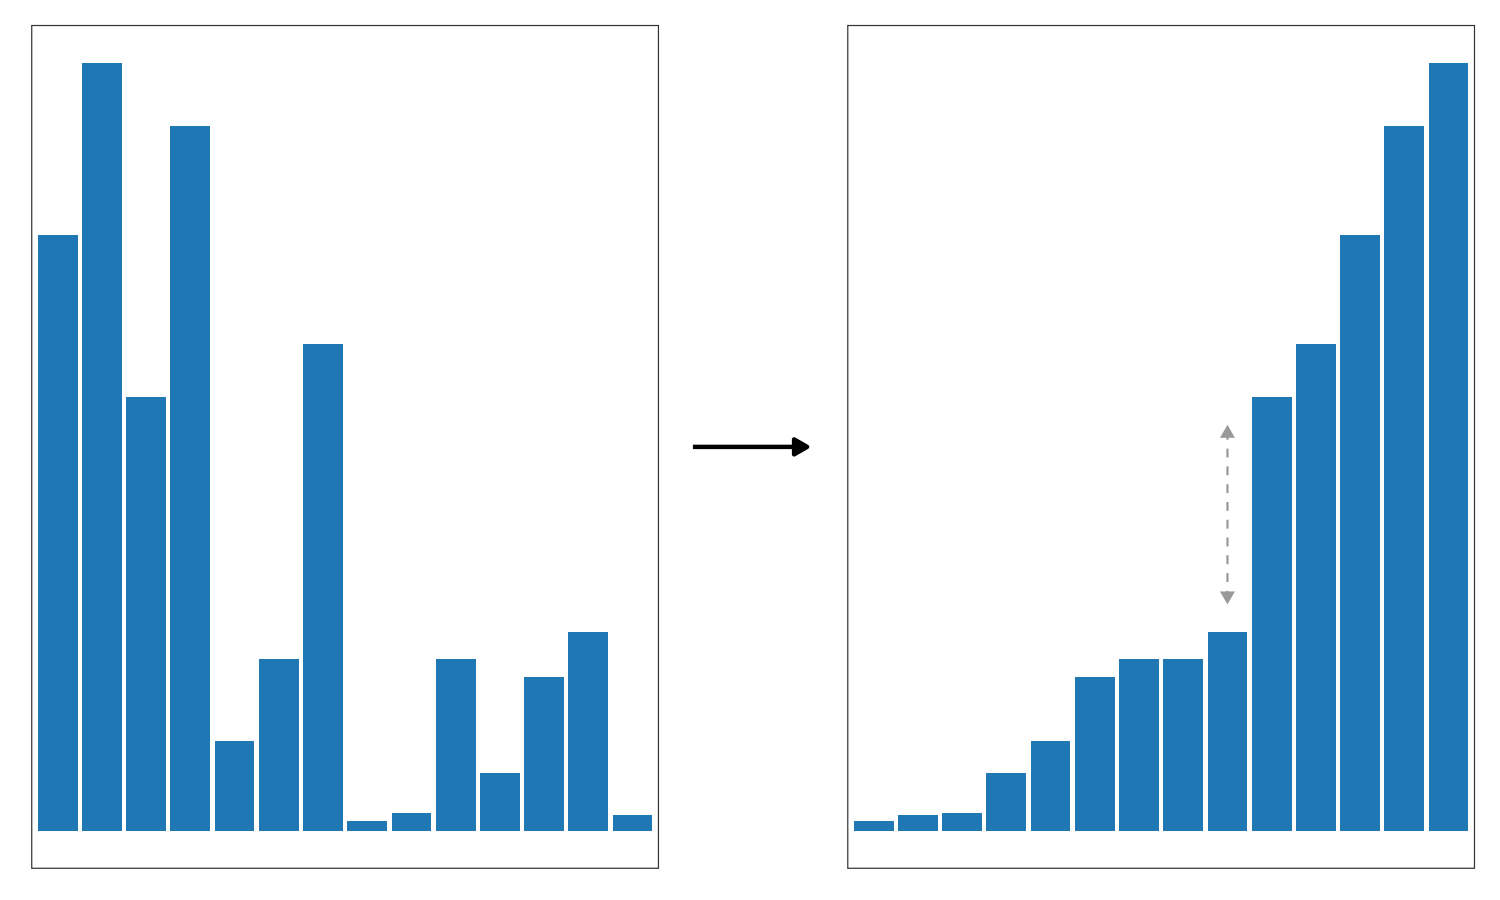
\includegraphics[width=20.83in]{./figures/sorting} 

}

\caption{Sorting or reordering can highlight interesting trends. For instance, sorting lexicographically ordered bars (left) by bar height (right) in the figure above immediately reveals a significant gap between the five tallest bars and the rest (gray dashed line).}\label{fig:sorting}
\end{figure}

There are more sophisticated ways to sort objects in a plot than just sorting bars by height, however. For instance, in plots which show multiple summary statistics, any may serve as the basis for the sorting rule; for instance a boxplot may be sorted by the median, upper and lower quartile, the maximum, and the minimum (\citeproc{ref-unwin2006}{Unwin et al. 2006}). Likewise, in the presence of selection/highlighting, objects may be sorted by the summary statistic on the highlighted parts. Alternatively, some systems allow users to permute the order of discrete scales manually by swapping the position of categories pairwise, a feature which can be particularly useful in parallel coordinate plots (\citeproc{ref-unwin2006}{Unwin et al. 2006}; \citeproc{ref-urbanek2011}{Urbanek 2011}). Finally, in the presence of many categories, sorting may also be usefully combined with lumping categories below a certain threshold together (\citeproc{ref-unwin2000}{Unwin 2000}).

Like zooming and panning, basic sorting typically involves the manipulation of axis scales only, making it also a fairly straightforward feature to implement. However, the more sophisticated sorting features can pose non-trivial implementation challenges (\citeproc{ref-unwin2006}{Unwin et al. 2006}). For instance, sorting by custom summary statistics or manually permuting discrete scale order may require specialized system components and behavior.

\subsubsection{Parametric interaction}\label{parametric-interaction}

As discussed in Section \ref{complexity-of-features}, another valuable class of interactive features are those which affect the computation of the summary statistics underlying the graphic (also called ``parametric interaction,'' \citeproc{ref-leman2013}{Leman et al. 2013}; \citeproc{ref-self2018}{Self et al. 2018}; \citeproc{ref-urbanek2011}{Urbanek 2011}). These features extend beyond simple manipulation of visual attributes, requiring that user interaction penetrates much deeper into the data visualization pipeline. Fundamentally, these features involve the manipulation of the parameters of some underlying mathematical model or algorithm.

An illustrative and popular example of parameter manipulation is dynamically changing histogram binwidth or anchor. Assuming a fixed binwidth \(w\) and an anchor \(a\), we can describe a histogram via a function \(h\) that, for each observation of a continuous variable \(x_i\) returns an index \(j\) of the corresponding bin, such that, for an ordered list of bins breaks \(b_j\), we have \(x_i \in [b_{j}, b_{j + 1})\)\footnote{Technically, if there are any values \(x_i < a\), we will have negative indices (\(j < 0\)), and if all values are significantly larger than the anchor, such that \(x_i > a + w\), the indices will not start at 1. So, to implement the histogram properly, we should shift all indices by subtracting the minimum index. Finally, if the histogram binwidth is not fixed, \(h\) becomes more complex as well.}:

\[h(x_i; a, w) = \lfloor (x_i - a) / w \rfloor + 1\]

Thus, a histogram really is a kind of a mathematical model, and can in fact be seen as a crude form of density estimation (see e.g. \citeproc{ref-bishop2006}{Bishop and Nasrabadi 2006, 4:120--22}). Manipulating histogram bins amounts to manipulating the parameters of the function \(h\). Crucially, unlike changes to surface-level visual attributes like size or opacity, changing binwidth or anchor requires recomputing the underlying summary statistics (\citeproc{ref-urbanek2011}{Urbanek 2011}). As noted in Section \ref{complexity-of-features}, these changes can have significant downstream effects. For instance, increasing the binwidth may cause certain bins to contain more data points than the current maximum, potentially requiring the adjustment of the upper y-axis limit, to prevent the bars from overflowing the plotting area.

There are other, more complex types of parametric interaction, than just changing histogram binwidth or anchor. These include, for example, modifying the bandwidth of a kernel density estimator, specifying the number of clusters in a clustering algorithm, or manipulating splitting criteria in classification and regression trees, as well as regularization parameters in smooth fits (for some more examples, see \citeproc{ref-leman2013}{Leman et al. 2013}; \citeproc{ref-self2018}{Self et al. 2018}).

Because parametric interaction necessitates recalculating the plot's underlying summary statistics, it is both more computationally expensive and as well as more difficult to implement. The interactive system must be able to respond to user input by recomputing relevant summaries and updating dependent plot parameters. In some systems such as Shiny (\citeproc{ref-shiny2024}{Chang et al. 2024}), the common approach is to re-render the entire plot from scratch each time any interaction occurs. However, this can become prohibitively expensive when these deep, parametric interactions are combined with rapid interactions closer to the surface of the visualization pipeline. Thus, the development of generic and efficient data visualization pipelines still remains an open research problem (\citeproc{ref-wickham2009}{Wickham et al. 2009}; \citeproc{ref-vanderplas2020}{Vanderplas, Cook, and Hofmann 2020}; \citeproc{ref-xie2014}{Xie, Hofmann, and Cheng 2014}).

\subsubsection{Animation and projection}\label{animation-and-projection}

A particularly useful form of parametric interaction involves the ability to control a continuous traversal through a series of states, observing the resulting changes as animation. This technique is especially useful when combined with projective techniques such as the grand tour (see \citeproc{ref-chen2008}{Chen et al. 2008}; for a recent comprehensive review, see \citeproc{ref-lee2022b}{Lee et al. 2022}), and for this reason I discuss them both here, within the same subsection.

A common and straightforward application of interactive animation is visualizing transitions in data subsets ordered by a specific variable, such as time. A particularly famous example of this technique is the \href{https://www.gapminder.org/tools/\#$chart-type=bubbles&url=v2}{interactive animation of the Gapminder data set} (\citeproc{ref-rosling2011}{Rosling and Zhang 2011}), which illustrates the joint evolution of GDP and life expectancy for countries worldwide. The interactive control of the timeline (play, pause, and pan) empowers users to explore time-dependent trends within this relatively high-dimensional data set, revealing trends that would be challenging to visualize by other means. For instance, the visualization clearly depicts the profound drop in both GDP and life expectancy during the second world war, followed by the subsequent rapid recovery and growth after 1945.

Interactive animation becomes particularly powerful when coupled with techniques like the grand tour (\citeproc{ref-asimov1985}{Asimov 1985}; \citeproc{ref-buja1986}{Buja and Asimov 1986}; \citeproc{ref-cook1995}{Cook et al. 1995}), designed for exploring high-dimensional datasets. Because data visualizations are typically limited to two dimensions, effectively representing high-dimensional data is challenging. The grand tour technique addresses this issue by projecting the data onto a series of lower-dimensional (two-dimensional) subspaces, interpolating between these projections, and animating the results to create a ``tour'' of different data views (\citeproc{ref-cook1995}{Cook et al. 1995}). By surveying this series of projections, the users may discover high-dimensional outliers, clusters, or non-linear dependencies (\citeproc{ref-wickham2011}{Wickham 2011}), and this discovery can be greatly aided by interactive controls of the animation's timeline or even manual control of the tour's direction (\citeproc{ref-chen2008}{Chen et al. 2008}; \citeproc{ref-lee2022b}{Lee et al. 2022}). Finally, the technique also integrates well with other interactive features, such as linked selection and querying/tooltips (\citeproc{ref-cook1995}{Cook et al. 1995}; \citeproc{ref-wickham2011}{Wickham 2011}; \citeproc{ref-lee2022a}{Lee, Laa, and Cook 2022}; \citeproc{ref-lee2022b}{Lee et al. 2022}).

The implementation complexity of interactive animation varies considerably depending on its application. While animating data subsets based on a single variable, as in the Gapminder visualization (\citeproc{ref-rosling2011}{Rosling and Zhang 2011}), presents no greater implementation challenges than previously discussed techniques, computing the grand tour path requires specialized algorithms (see, e.g., \citeproc{ref-chen2008}{Chen et al. 2008}, for a brief description). However, if the data subsets corresponding to each animation frame are pre-computed, the animation itself is generally fairly straightforward to implement.

\subsubsection{Representation switching}\label{representation-switching}

Another specialized kind of parametric (or semi-parametric) interaction involves changing the representation of the underlying data. It is well known that the same data can often be visualized using various sets of visual encodings (\citeproc{ref-wilkinson2012}{Wilkinson 2012}), with some being more effective for answering specific questions than others. Enabling users to switch between these various representations provides greater flexibility for data exploration (\citeproc{ref-yi2007}{Yi et al. 2007}). However, for certain plot types, changing the representation involves more than just altering surface-level visual attributes; it also necessitates recalculating derived statistics.

A typical example is switching between a barplot and a spineplot, see Figure \ref{fig:barplot-spineplot1}. Barplots are effective for comparing absolute quantities. Specifically, by encoding categories along the x-axis and continuous quantities along the y-axis (bar height), we can easily compare the quantities across categories. Color-coding parts of the bars as segments allows us to visualize a second categorical variable, enabling subgroup comparisons of absolute values. However, barplots are less well-suited for comparing the \emph{proportions} represented by these segments, particularly when bar heights vary considerably.

\begin{figure}

{\centering 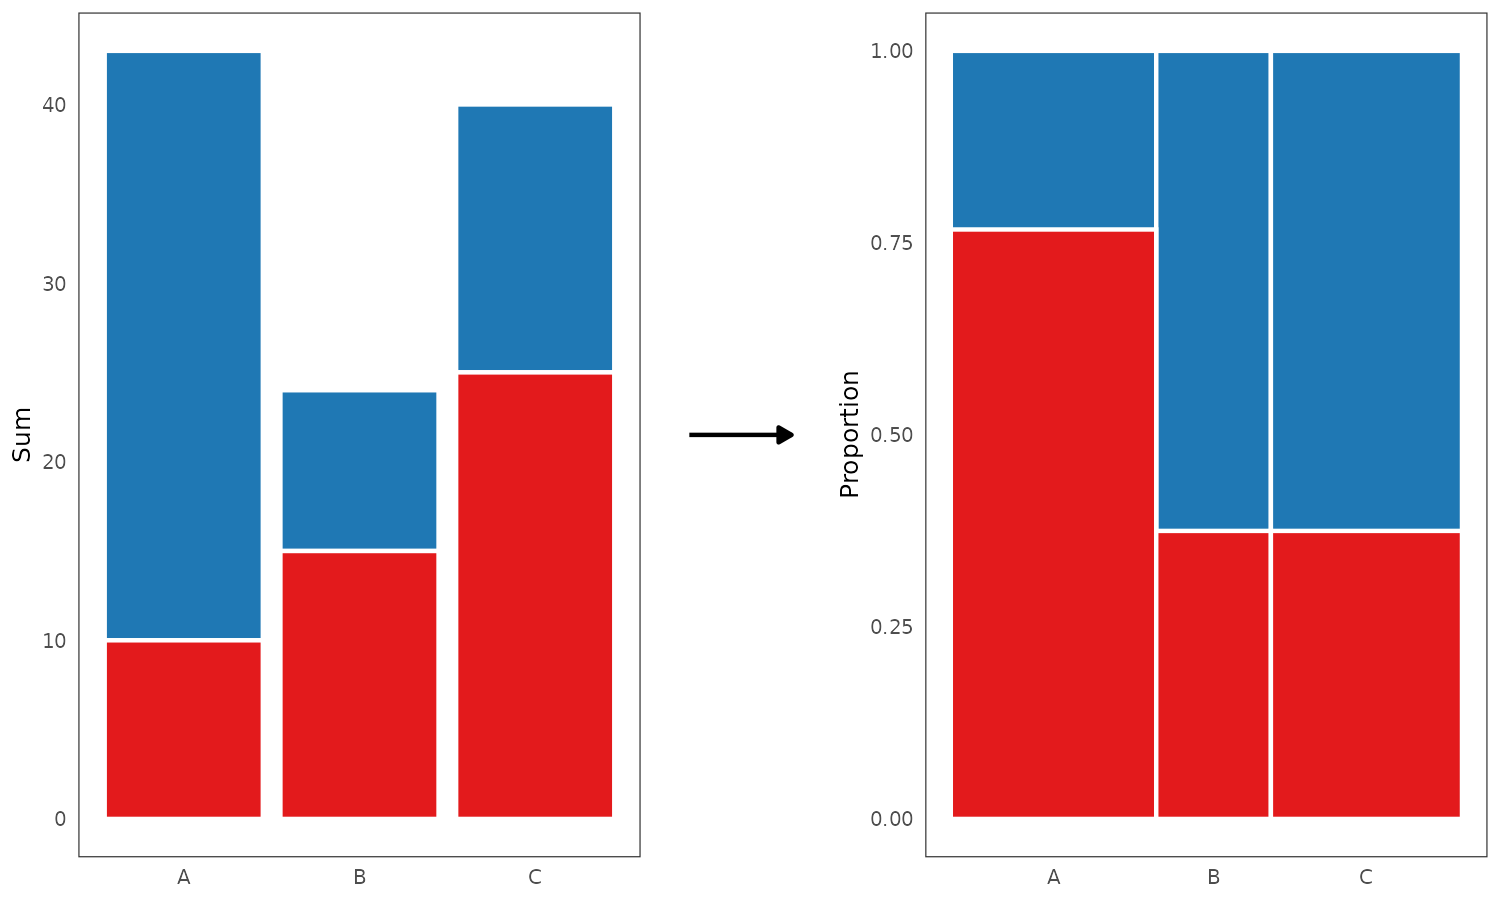
\includegraphics[width=20.83in]{./figures/barplot-spineplot} 

}

\caption{Switching representation can be an effective way to derive new insights from the data. A barplot (left) represents the same underlying data as a spineplot (right), however, the former is better for comparing absolute counts whereas the latter is better for comparing proportions. Note that in the spineplot, it is much easier to see that the proportion of the red cases is the same in categories B and C.}\label{fig:barplot-spineplot1}
\end{figure}

Spineplots, on the other hand, present a way of visualizing the same sort of data as a barplot while making it much easier to compare proportions. Specifically, in a spineplot, the heights of the bars are all normalized to 1, such that the segments show a proportion of the total, and the original values are instead encoded as the bar width, which is stacked along the x-axis. Thus, the fixed height of bars makes it easy to compare the segments proportionally.

Other examples of switching of representations include switching from a histogram to spinogram (a normalized version of the histogram) and switching between aggregate geometric objects and individual points (e.g.~boxplot, parallel coordinate plots).

\subsubsection{Linked selection}\label{linked-selection}

Linked selection, also known as linked brushing, linked highlighting, or linked views, is often considered one of the most versatile and powerful interactive data visualization features (see e.g. \citeproc{ref-becker1987}{Becker and Cleveland 1987}; \citeproc{ref-buja1996}{Buja, Cook, and Swayne 1996}; \citeproc{ref-wilhelm2003}{Wilhelm 2003}; \citeproc{ref-heer2012}{Heer and Shneiderman 2012}; \citeproc{ref-ward2015}{Ward, Grinstein, and Keim 2015}; \citeproc{ref-ware2019}{Ware 2019}). Fundamentally, it involves creating a figure with multiple ``linked'' plots. The user can then click or click-and-drag over objects in one plot, and the corresponding cases are highlighted across all the other plots, see Figure \ref{fig:linked-selection}. This makes it possible to quickly quickly explore trends across different dynamically-generated subsets of the data (\citeproc{ref-dix1998}{Dix and Ellis 1998}). The ability to quickly materialize alternative views of the data makes this a particularly effective tool for data exploration (\citeproc{ref-wilhelm2008}{Wilhelm 2008}; \citeproc{ref-wills2008}{G. Wills 2008}).

\begin{figure}

{\centering 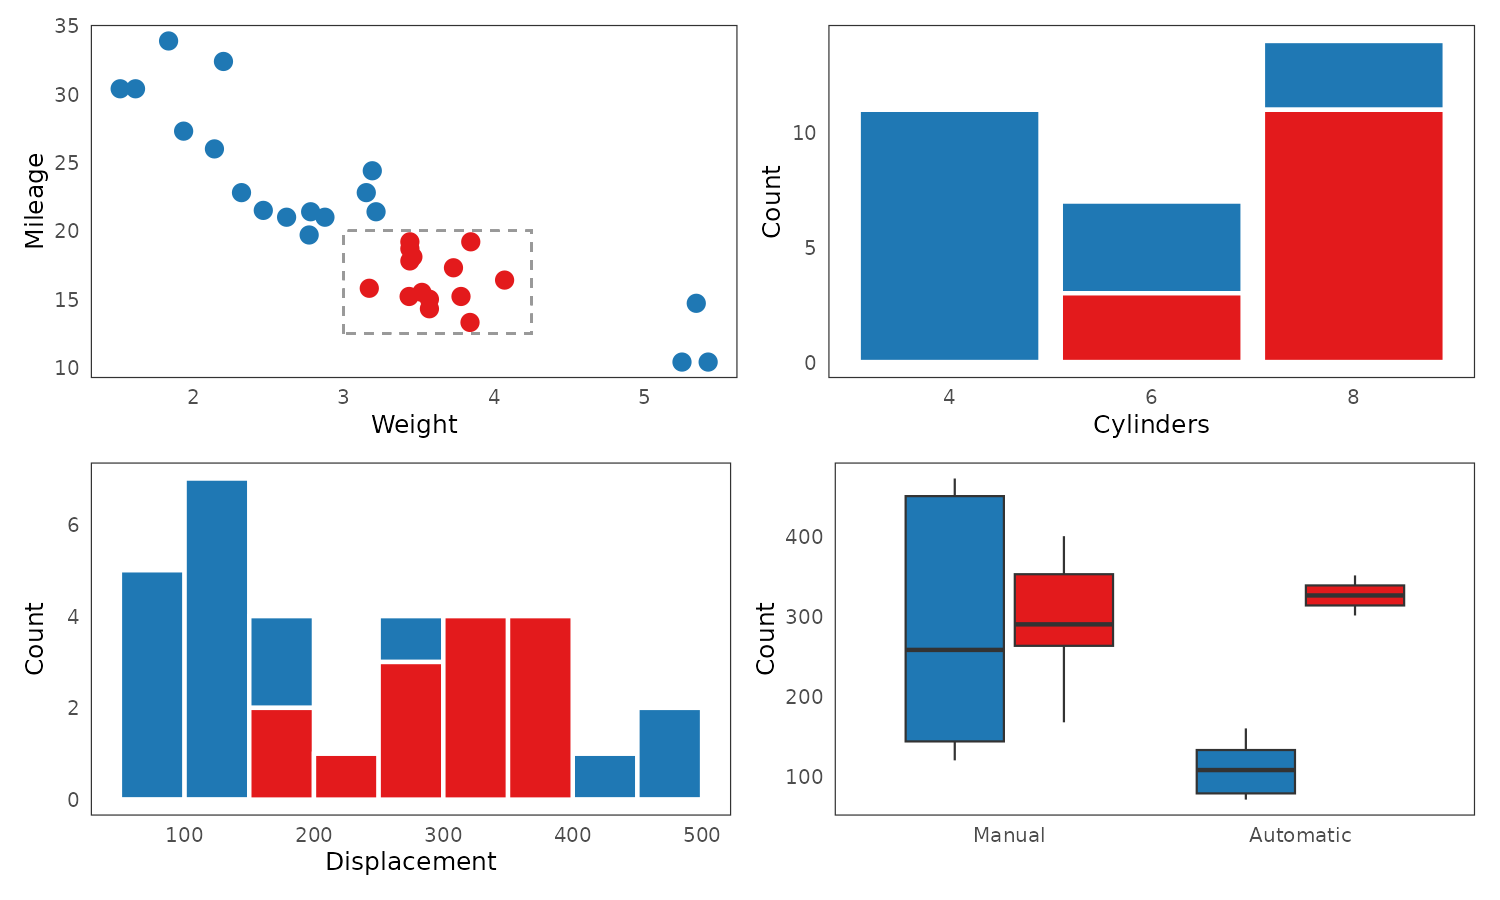
\includegraphics[width=20.83in]{./figures/linked-selection} 

}

\caption{Linked selection involves highlighting the same cases across all plots. The user can select some objects in one plot, such as points in a scatterplot (top left), and the corresponding cases are higlighted in all the other plots. Source of the underlying data is the `mtcars` dataset [@henderson1981].}\label{fig:linked-selection}
\end{figure}

Despite the fact that the user experience of linked selection is usually fairly intuitive, there are many subtle considerations that go into implementing the feature (for a good overview, see \citeproc{ref-wilhelm2008}{Wilhelm 2008}). First, there is the issue of how the user makes the selection. Typically, clicking selects a single objects and clicking-and-dragging selects multiple objects in a rectangular region (similar to how selecting files and folders works on desktop GUIs of most operating systems). In some systems, the users may also drag the selection region around (``brushing''), form a continuous ``lasso'' selection, select lines in a particular angular range, or points at a particular distance from a centroid (see e.g. \citeproc{ref-hauser2002}{Hauser, Ledermann, and Doleisch 2002}; \citeproc{ref-splechtna2018}{Splechtna et al. 2018}; \citeproc{ref-wills2008}{G. Wills 2008}). Further, when one variables is continuous and the other is derived (such as the x- and y-axes in a histogram), the interaction may also be simplified by restricting selection/brushing to the primary axis (\citeproc{ref-satyanarayan2016}{Satyanarayan et al. 2016}). Finally, the selections can be combined by various operators such as OR, AND, NOT, and XOR, to form unions, intersections, and other types of logical subsets (\citeproc{ref-theus2002}{Theus 2002}; \citeproc{ref-urbanek2003}{Urbanek and Theus 2003}; \citeproc{ref-wills2000}{G. J. Wills 2000}; \citeproc{ref-wills2008}{G. Wills 2008}).

Second, there is the issue of who should dispatch and respond to selection events. In presentation-focused interactive data visualization and dashboarding systems, this responsibility is kept flexible, such that some plots may only dispatch, only respond, do both, or neither (\citeproc{ref-satyanarayan2015}{Satyanarayan et al. 2015}, \citeproc{ref-satyanarayan2016}{2016}). However, in systems focused on data exploration, the convention is typically for all plots to both dispatch and respond to selection events, such that they may be interacted with in the same way. (\citeproc{ref-theus2002}{Theus 2002}; \citeproc{ref-urbanek2003}{Urbanek and Theus 2003}; \citeproc{ref-urbanek2011}{Urbanek 2011}).

Third, there is the issue of what to link. In the case of data represented by a two-dimensional table or data frame, the most common method is to link cases taken on the same observational level (identity linking), such that each row gets assigned a value representing the selection status (\citeproc{ref-urbanek2003}{Urbanek and Theus 2003}; \citeproc{ref-wilhelm2008}{Wilhelm 2008}; \citeproc{ref-wills2008}{G. Wills 2008}). However, in the case of more complex data, more advanced linking schemes are also available, such as hierarchical and distance-based linking (\citeproc{ref-wilhelm2008}{Wilhelm 2008}; \citeproc{ref-urbanek2011}{Urbanek 2011}).

Third, there is the issue of displaying selection. This issue will be touched upon in more detail later, in Section \ref{problems}. Briefly, Wilhelm (\citeproc{ref-wilhelm2008}{2008}) identifies three methods for displaying linked selection: replacement, overlaying, and repetition. Replacement involves replacing the entire plot with a new graphic; overlaying involves superimposing the objects representing the selected subsets on top of the original objects; and repetition involves displaying the selected objects alongside the original ones. Wilhelm identifies issues with all three techniques, although he does seem to generally come down in favor of repetition (however, see my argument in Section \ref{stacking-part-whole}).

A fourth and final issue in linked selection, and arguably one of the core concerns of the present thesis, is consistency. This topic will be coming up again and again, particularly in Section \ref{problems}. Consistent and predictable features are a cornerstone of good user interface design (see e.g. \citeproc{ref-ruiz2021}{Ruiz, Serral, and Snoeck 2021}). However, as discussed above, the design an interactive data visualization system supporting linked selection presents many design decisions, each with its own set of implementation constraints. Achieving a consistent user interface through the right combination of these decisions is a known challenge (\citeproc{ref-urbanek2011}{Urbanek 2011}; \citeproc{ref-pike2009}{Pike et al. 2009}).

For example, while the approach of allowing objects to independently dispatch and display selection events offers great flexibility, it can also lead to a less intuitive user experience. Put simply, when users select objects in one linked plot by clicking them, they might reasonably expect the same functionality in other plots. If that is not the case (if, for instance, other plots support only displaying but not dispatching selection events), their expectation will be violated. Thus, it might be reasonable to require that all objects can both dispatch and display selection events. However, this places some fundamental constraints on these objects. For instance, how do we draw a lineplot line where only some of the underlying cases are selected? Do we draw a sequence of differently-coloured line segments, leading to a striped ``candy cane'' pattern (see Figure \ref{fig:line-consistency})? Do we draw two separate lines? If so, how do we then dispatch selection events on these lines which are already conditional on selection? Like turning over a rock and disturbing a host of creepy-crawlies, linked selection reveals a complex web of visualization design challenges that defy a satisfying, generic solution.

\begin{figure}

{\centering 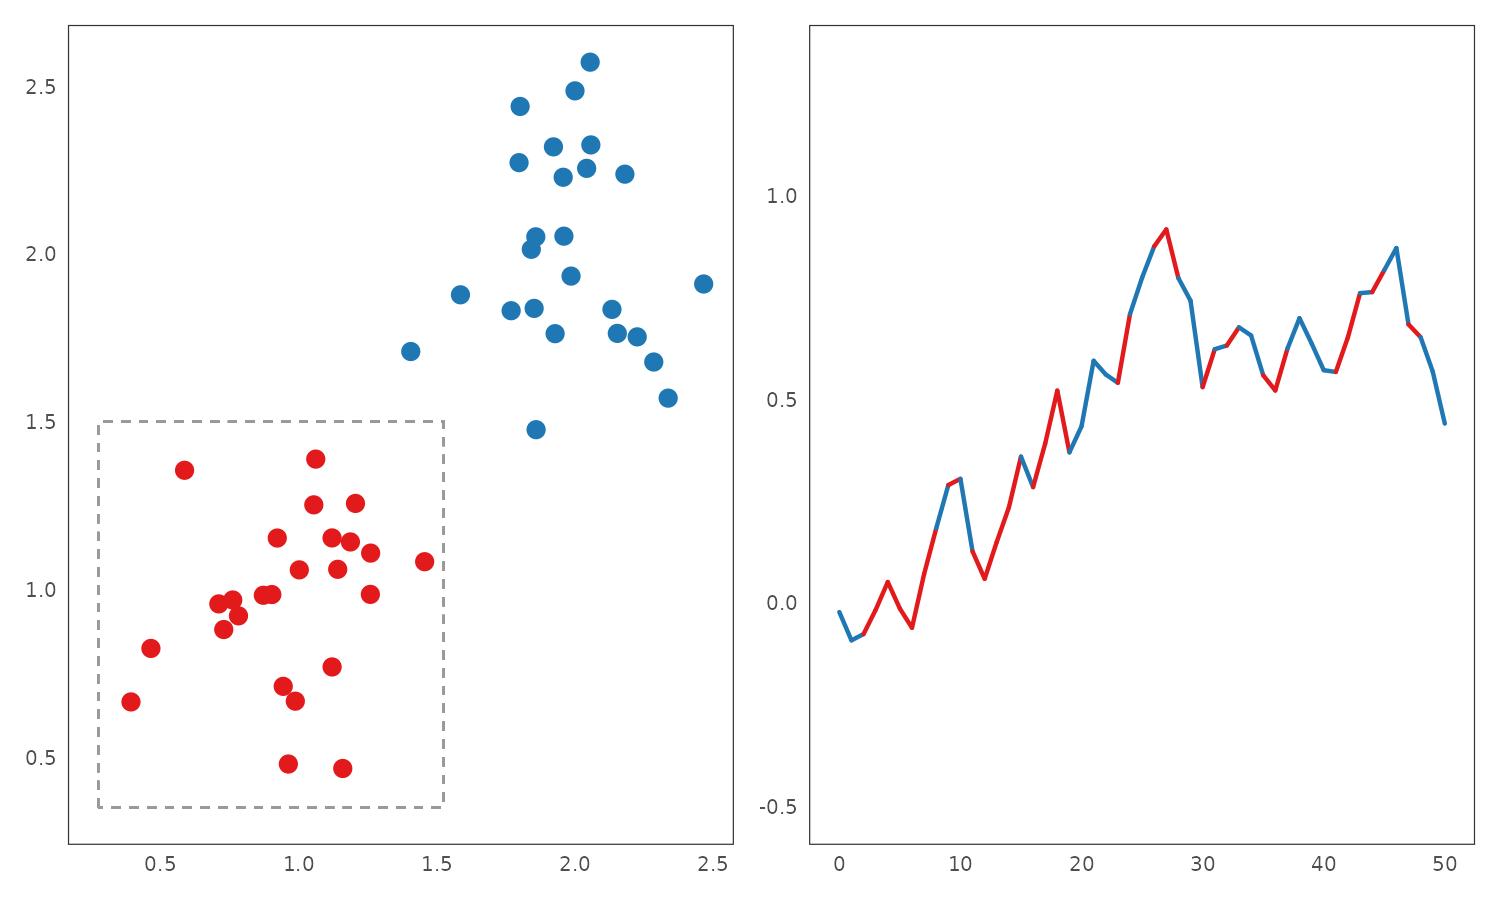
\includegraphics[width=20.83in]{./figures/line-consistency} 

}

\caption{Displaying selection is not always trivial. A good example is a lineplot (right). Whereas a point in a scatterplot displays a single case (row) and a bar in a barplot displays a simple subset of cases, a line segment in a lineplot connects two data points. As such, it is not clear whether to highlight the segment *starting* at the selected point, *ending* at the selected point, or, e.g., half a segment on each side of the point. Further, since the geometry of a segmented line is not commutative (row order matters), we end up with a striped 'candy cane' pattern that is not easily interpretable.}\label{fig:line-consistency}
\end{figure}

\section{General data visualization theory}\label{general-data-visualization-theory}

The following sections briefly explore several key theoretical topics in data visualization: the goals and purpose of visualizations, the mechanisms of visual perception, and the theory of scales and measurement. While mainly discussed in the context of static visualization, these topics are equally relevant to interactive visualization and present some unique challenges. My goal is not to give an exhaustive review - each of these topics is substantial enough to serve as a thesis topic in its own right. Instead, I just want to give a brief overview of these topics, highlight some key points, and discuss how they may relate to my own work.

\subsection{Visualization goals}\label{visualization-goals}

An important fact about data visualization is that, fundamentally, a chart can be used by many different people for many different things (for a review, see e.g. \citeproc{ref-brehmer2013}{Brehmer and Munzner 2013}; \citeproc{ref-franconeri2021}{Franconeri et al. 2021}; \citeproc{ref-sarikaya2018}{Sarikaya et al. 2018}). For example, applied researchers may create figures as part of their workflow, aiming to better understand the data they had collected, spot errors and anomalies, and come up with new ideas and hypotheses (\citeproc{ref-brehmer2013}{Brehmer and Munzner 2013}; see also \citeproc{ref-kandel2012}{Kandel et al. 2012}). Conversely, data scientists and data analysts in the public and private sector may visualize already familiar data sets to communicate important information, drive decisions, or convince or persuade stakeholders (\citeproc{ref-sarikaya2018}{Sarikaya et al. 2018}). Finally, some figures may be created out of a sense of curiosity or for pure aesthetic enjoyment (\citeproc{ref-brehmer2013}{Brehmer and Munzner 2013}; \citeproc{ref-tufte2001}{Tufte 2001}). Depending on the end-goals of the user and the desired target audience, certain visualization techniques, methods, or styles may become more useful than others.

As mentioned in Section \ref{interactive-interacting}, much has been written about the goals and experiences a user might have while creating data visualizations. For instance, Brehmer and Munzner (\citeproc{ref-brehmer2013}{2013}) formalized a typology of abstract visualization tasks, based around three adverbs: \emph{why} is a task is performed, \emph{how} it is performed, and \emph{what} does it pertain to. In the \emph{why} part of their typology, they list the following reasons for why a user may engage in the process of visualizing data: to consume (present, discover, or enjoy), produce, search (lookup, browse, locate, and explore), and query (identify, compare, summarize). As another example, Pike et al. (\citeproc{ref-pike2009}{2009}) list the following high-level goals a user might have when interacting with a visualization: explore, analyze, browse, assimilate, triage, asses, understand, compare. And there are many other typologies and taxonomies of data visualization tasks and goals in the literature.

Personally, when it comes to classifying interactive data visualization goals, I prefer the following short list provided by Ward, Grinstein, and Keim (\citeproc{ref-ward2015}{2015}):

\begin{itemize}
\tightlist
\item
  Exploration: The user wants to examine a data set
\item
  Confirmation: The user wants to verify a fact or a hypothesis
\item
  Presentation: The user wants to use the visualization to convince or inspire an audience
\item
  Interactive presentation: The user wants to take the audience on a guided tour of key insights
\end{itemize}

I believe this list maps fairly well onto interactive data visualization systems found in the wild, such as the ones discussed in Section \ref{brief-history}. Specifically, as mentioned before, in the history of interactive data visualization, the earlier statistical systems seemed to primarily focus on exploration and confirmation, whereas the newer web-based systems seem to prioritize presentation. The interactive presentation category is interesting, since, I would argue, it is far more specific and less common than the other categories, however, by singling it out, Ward et al.~make an interesting point. By incorporating time and intentionality, sequential interactive presentations, such as those found in the Graphics section of the New York Times (\citeproc{ref-nytimes2025}{The New York Times Company 2025}), really are quite unique.

\subsection{Visual perception}\label{visual-perception}

Another important research topic in data visualization is visual perception. Specifically, given that we use visual attributes such as position, color, length, or area to encode various aspects of our data, researchers have tried to answer the question of how to use these attributes in a way that best leverages the human visual system. Fortunately, this research has been quite fruitful, yielding precise and actionable guidelines (for a review, see \citeproc{ref-franconeri2021}{Franconeri et al. 2021}; \citeproc{ref-quadri2021}{Quadri and Rosen 2021}).

A landmark work in this area has been that of Cleveland and McGill (\citeproc{ref-cleveland1984}{1984}). In this study, the authors conducted a series of empirical experiments in which they investigated people's ability to accurately judge quantities based on different visual encodings. They found that judgments based on position along a common scale were the most accurate, followed by length-based comparisons, and then angle-based comparisons.

The findings were later corroborated by other authors. Heer and Bostock (\citeproc{ref-heer2010}{2010}) replicated the Cleveland and McGill (\citeproc{ref-cleveland1984}{1984}) study, and included judgements of circular and rectangular areas which were found to be less accurate than position, length, or angle. Other authors have extended these experiments to other visual encodings, such as color or density (e.g. \citeproc{ref-demiralp2014}{Demiralp, Bernstein, and Heer 2014}; \citeproc{ref-saket2017}{Saket et al. 2017}; \citeproc{ref-reda2018}{Reda, Nalawade, and Ansah-Koi 2018}). Together, these findings have been used to create rankings of visual encodings, with researchers generally agreeing on the following ordered list: position, length, area, angle, and intensity (from most effective to least, \citeproc{ref-mackinlay1986}{Mackinlay 1986}; \citeproc{ref-franconeri2021}{Franconeri et al. 2021}; \citeproc{ref-quadri2021}{Quadri and Rosen 2021}).

\subsection{Scales and measurement}\label{scales-measurement}

Visualizing data involves mapping values to graphical attributes. As discussed in the previous section, certain visual attributes are better for visualizing particular types of data, and vice versa. However, even when we pick an appropriate visual attribute to represent our data with, there are still many choices in how to perform the mapping. For instance, suppose we have some variable \(x\) with values \(\{ 1, 2, 3 \}\). Should these be treated as magnitudes, a simple ordering, or even just category labels that may be permuted at will? In most data visualization systems, this metadata encoding of values into visual attributes is handled specialized components called scales or coordinate systems, and I will discuss their implementation in detail later, in Section \ref{scales-composition}. However, it is first necessary to discuss some theoretical issues involving scales.

A particular challenge when discussing scales in data visualization is that the topic unavoidably intersects with a research area that has a particularly long and contentious history: theory of measurement (see e.g. \citeproc{ref-hand1996}{Hand 1996}; \citeproc{ref-michell1986}{Michell 1986}; \citeproc{ref-tal2025}{Tal 2025}). Theory of measurement (not to be confused with measure theory, with which it nevertheless shares some overlap) is the research area which tries to answer the deceptively simple question: what does it mean to measure something? This seemingly trivial problem has inspired long and fiery debates within the fields of mathematics, philosophy, and social science. Particularly, in psychology, where assigning numerical values non-physical phenomena such as moods and mental states is a central concern, the topic has garnered a significant amount of attention, creating a dense body of research (see e.g. \citeproc{ref-humphry2013}{Humphry 2013}; \citeproc{ref-michell2021}{Michell 2021}).

Arguably, the most influential work in this field has been that of Stevens (\citeproc{ref-stevens1946}{1946}). In his fairly concise paper, Stevens defined a \emph{scale} as method of assigning numbers to values, and introduced a four-fold classification classification, namely: nominal, ordinal, interval, and ratio scales (see Table \ref{tab:stevens-scales}).

\begin{table}

\caption{\label{tab:stevens-scales}Types of scales identified by Stevens (1946)}
\centering
\begin{tabular}[t]{l|l|l|l}
\hline
Scale & Structure & Comparison & Valid transformations\\
\hline
Nominal & Isomorphism & Are \$x\$ and \$y\$ the same? & \$x' = f(x)\$, where \$f\$ is a bijection\\
\hline
Ordinal & Monotone map & Is \$x\$ is greater than \$y\$? & \$x' = f(x)\$, where \$f\$ is a monotone bijection\\
\hline
Interval & Affine transformation & How far is \$x\$ from \$y\$? & \$x' = ax + b\$, for \$a, b \textbackslash{}in \textbackslash{}mathbb\{R\}\$\\
\hline
Ratio & Linear map & How many times is \$x\$ greater than \$y\$? & \$x' = ax\$, for \$a \textbackslash{}in \textbackslash{}mathbb\{R\}\$\\
\hline
\end{tabular}
\end{table}

The Steven's (\citeproc{ref-stevens1946}{1946}) typology is based on invariance under transformation. Specifically, for each class of scales, we define a set of transformations that preserve valid comparisons. The set of valid transformations shrinks as we move from one class of scales to another.

For nominal scales, any kind of bijective transformation is valid. Intuitively, we can think of the scale as assigning labels to values, and any kind re-labeling is valid, as long as it preserves equality of the underlying values. For instance, given a nominal scale with three values, we can assign the labels \(\{ \text{red}, \text{green}, \text{blue} \}\) or \(\{ \text{monday}, \text{tuesday}, \text{wednesday} \}\) in any way we like, as long as each value maps to a unique label. This identifies the underlying mathematical structure as an isomorphism.

Ordinal scales are more restrictive, since, on top of preserving equality, transformations also need to preserve order. For example, if we want to assign the labels \(\{ \text{monday}, \text{tuesday}, \text{wednesday} \}\) to an ordinal scale with three values, there is only one way to do it that preserves the underlying order: assign the least values to \(\text{monday}\), the middle value to \(\text{tuesday}\), and the greatest value to \(\text{wednesday}\) (assuming we order the labels/days in the usual day-of-week order). However, there is no notion of distance between the labels: we could just as well assign the values labels in \(\mathbb{N}\) such as \(\{ 10, 20, 30 \}\), \(\{1, 2, 9999 \}\), and so on. Thus, the fundamental mathematical structure is that of a monotone map.

Interval scales need to additionally preserve equality of intervals. This means that, for any three values \(a, b,\) and \(c\), if the distances between \(a\) and \(b\) and \(b\) and \(c\) are equal, \(d(a, b) = d(b, c)\), then so should be the distances between the scaled labels, \(d^*(f(a), f(b)) = d^*(f(b), f(c)\). For most real applications, this limits interval scales to the class of affine transformations of the form \(f(x) = ax + b\). A canonical example of an interval scale is the conversion formula of degrees Celsius to Fahrenheit: \(f(c) = 9/5 \cdot c + 32\) (\citeproc{ref-stevens1946}{Stevens 1946}). This example also highlights an important property of interval scales: the zero point can be arbitrary and ratios are not meaningful. Specifically, since the zero points of both Celsius and Fahrenheit scales were chosen based on arbitrary metrics (freezing temperatures of water and brine, respectively), it does not make sense to say that, e.g.~20°C is ``twice as hot'' as 10°C, in the same way that it does not make sense to say that 2000 CE is ``twice as late'' as 1000 CE.

Finally, ratio scales also need to preserve the equality of ratios. Specifically, if \(a/b = b/c\) then \(f(a)/f(b) = f(b) / f(c)\). As a consequence, this also means that the scale must have a well-defined zero-point. Examples of ratio scales include physical magnitudes such as height and weight, which have a well-defined zero point (\citeproc{ref-stevens1946}{Stevens 1946}).

Steven's (\citeproc{ref-stevens1946}{1946}) typology sparked a considerable debate, on multiple fronts. First, since the original publication, many authors have sought to either expand upon or criticize Steven's typology. However, despite some monumental efforts towards a unified theory, such as that of Krantz et al. (\citeproc{ref-krantz1971}{1971}), measurement has remained a hotly debated topic to this day (see e.g. \citeproc{ref-michell2021}{Michell 2021}; \citeproc{ref-tal2025}{Tal 2025}). Second, more relevant to statistics, some authors such as Stevens (\citeproc{ref-stevens1951}{1951}) and Luce (\citeproc{ref-luce1959}{1959}) used the theory to define come up with prescriptive rules for statistical transformations, suggesting that, for example, taking the mean of an ordinal variable is wrong since the meaning of the average operator is not preserved under monotone transformations. However, this issue was hotly contested by statisticians such as Lord (\citeproc{ref-lord1953}{1953}), Tukey (\citeproc{ref-tukey1986}{1986}), and Velleman and Wilkinson (\citeproc{ref-velleman1993}{1993}), who argued that many well-established statistical practices, such as rank-based tests and coefficients of variations, rely on such ``impermissible'' statistics but can nevertheless yield valuable insights. More broadly, these authors also argued that data is not really meaningful on its own, but instead derives its meaning from the statistical questions it is used to answer (see also \citeproc{ref-wilkinson2012}{Wilkinson 2012}).

At this point, the discussion around measurement has arguably become far too dense and theoretical, and most data visualization researchers seem to avoid delving into it too deeply (see e.g. \citeproc{ref-wilkinson2012}{Wilkinson 2012}). Nevertheless, there are still some areas where the issues of measurement and Steven's typology do crop up. For instance, when scaling area based on a continuous variable, a common recommendation is to start the scale at zero to ensure accurate representations of ratios (see e.g. \citeproc{ref-wickham2024}{Wickham and Navarro 2024}), aligning with Steven's definition of a ratio scale. Likewise, the long-standing debate around whether the base of a barplot should always start at zero (see e.g. \citeproc{ref-cleveland1985}{Cleveland 1985}; \citeproc{ref-wilkinson2012}{Wilkinson 2012}) also carries echoes of the measurement debate. Ultimately, it may yet require long time to settle the issues around measurement, however, there are definitely some ideas within the literature that data visualization can benefit from.

\phantomsection\label{refs}
\begin{CSLReferences}{1}{0}
\bibitem[\citeproctext]{ref-abbate1999}
Abbate, J. 1999. {``{Getting small: a short history of the personal computer}.''} \emph{Proc. IEEE} 87 (9): 1695--98. \url{https://doi.org/10.1109/5.784256}.

\bibitem[\citeproctext]{ref-abukhodair2013}
Abukhodair, Felwa A, Bernhard E Riecke, Halil I Erhan, and Chris D Shaw. 2013. {``Does Interactive Animation Control Improve Exploratory Data Analysis of Animated Trend Visualization?''} In \emph{Visualization and Data Analysis 2013}, 8654:211--23. SPIE.

\bibitem[\citeproctext]{ref-asimov1985}
Asimov, Daniel. 1985. {``The Grand Tour: A Tool for Viewing Multidimensional Data.''} \emph{SIAM Journal on Scientific and Statistical Computing} 6 (1): 128--43.

\bibitem[\citeproctext]{ref-backus1978}
Backus, John. 1978. {``The History of Fortran i, II, and III.''} \emph{ACM Sigplan Notices} 13 (8): 165--80.

\bibitem[\citeproctext]{ref-batch2017}
Batch, Andrea, and Niklas Elmqvist. 2017. {``The Interactive Visualization Gap in Initial Exploratory Data Analysis.''} \emph{IEEE Transactions on Visualization and Computer Graphics} 24 (1): 278--87.

\bibitem[\citeproctext]{ref-becker1987}
Becker, Richard A, and William S Cleveland. 1987. {``Brushing Scatterplots.''} \emph{Technometrics} 29 (2): 127--42.

\bibitem[\citeproctext]{ref-beniger1978}
Beniger, James R, and Dorothy L Robyn. 1978. {``Quantitative Graphics in Statistics: A Brief History.''} \emph{The American Statistician} 32 (1): 1--11.

\bibitem[\citeproctext]{ref-bertin1967}
Bertin, Jacques. 1967. \emph{{Sémiologie Graphique: Les diagrammes, les réseaux, les cartes}}. Gauthier-Villars.

\bibitem[\citeproctext]{ref-bishop2006}
Bishop, Christopher M, and Nasser M Nasrabadi. 2006. \emph{Pattern Recognition and Machine Learning}. Vol. 4. 4. Springer.

\bibitem[\citeproctext]{ref-flare2020}
Blokt. 2020. {``Flare {\(\vert\)} Data Visualization for the Web.''} \emph{Blokt - Privacy, Tech, Bitcoin, Blockchain {\&} Cryptocurrency}. \url{https://blokt.com/tool/prefuse-flare}.

\bibitem[\citeproctext]{ref-bostock2022}
Bostock, Mike. 2022. {``D3.js - Data-Driven Documents.''} \url{https://d3js.org}.

\bibitem[\citeproctext]{ref-bracsoveanu2017}
Braşoveanu, Adrian MP, Marta Sabou, Arno Scharl, Alexander Hubmann-Haidvogel, and Daniel Fischl. 2017. {``Visualizing Statistical Linked Knowledge for Decision Support.''} \emph{Semantic Web} 8 (1): 113--37.

\bibitem[\citeproctext]{ref-brasseur2005}
Brasseur, Lee. 2005. {``Florence Nightingale's Visual Rhetoric in the Rose Diagrams.''} \emph{Technical Communication Quarterly} 14 (2): 161--82.

\bibitem[\citeproctext]{ref-brehmer2013}
Brehmer, Matthew, and Tamara Munzner. 2013. {``A Multi-Level Typology of Abstract Visualization Tasks.''} \emph{IEEE Transactions on Visualization and Computer Graphics} 19 (12): 2376--85.

\bibitem[\citeproctext]{ref-brodbeck2009}
Brodbeck, Dominique, Riccardo Mazza, and Denis Lalanne. 2009. {``{Interactive Visualization - A Survey}.''} In \emph{{Human Machine Interaction}}, 27--46. Berlin, Germany: Springer. \url{https://doi.org/10.1007/978-3-642-00437-7_2}.

\bibitem[\citeproctext]{ref-buja1986}
Buja, Andreas, and Daniel Asimov. 1986. {``Grand Tour Methods: An Outline.''} In \emph{Proceedings of the Seventeenth Symposium on the Interface of Computer Sciences and Statistics on Computer Science and Statistics}, 63--67.

\bibitem[\citeproctext]{ref-buja1996}
Buja, Andreas, Dianne Cook, and Deborah F Swayne. 1996. {``Interactive High-Dimensional Data Visualization.''} \emph{Journal of Computational and Graphical Statistics} 5 (1): 78--99.

\bibitem[\citeproctext]{ref-cairo2014}
Cairo, Alberto. 2014. {``Graphics Lies, Misleading Visuals: Reflections on the Challenges and Pitfalls of Evidence-Driven Visual Communication.''} In \emph{New Challenges for Data Design}, 103--16. Springer.

\bibitem[\citeproctext]{ref-cairo2019}
---------. 2019. \emph{How Charts Lie: Getting Smarter about Visual Information}. WW Norton \& Company.

\bibitem[\citeproctext]{ref-shiny2024}
Chang, Winston, Joe Cheng, JJ Allaire, Carson Sievert, Barret Schloerke, Yihui Xie, Jeff Allen, Jonathan McPherson, Alan Dipert, and Barbara Borges. 2024. \emph{Shiny: Web Application Framework for r}. \url{https://CRAN.R-project.org/package=shiny}.

\bibitem[\citeproctext]{ref-chen2008}
Chen, Chun-houh, Wolfgang Härdle, Antony Unwin, Dianne Cook, Andreas Buja, Eun-Kyung Lee, and Hadley Wickham. 2008. {``Grand Tours, Projection Pursuit Guided Tours, and Manual Controls.''} \emph{Handbook of Data Visualization}, 295--314.

\bibitem[\citeproctext]{ref-clark2017}
Clark, Lin. 2017. {``A Crash Course in Just-in-Time (JIT) Compilers.''} \emph{Mozilla Hacks {\textendash} the Web Developer Blog}. \url{https://hacks.mozilla.org/2017/02/a-crash-course-in-just-in-time-jit-compilers}.

\bibitem[\citeproctext]{ref-clayton2021}
Clayton, Aubrey. 2021. \emph{Bernoulli's Fallacy: Statistical Illogic and the Crisis of Modern Science}. Columbia University Press.

\bibitem[\citeproctext]{ref-cleveland1985}
Cleveland, William S. 1985. \emph{The Elements of Graphing Data}. Wadsworth Publ. Co.

\bibitem[\citeproctext]{ref-cleveland1993}
---------. 1993. \emph{Visualizing Data}. Hobart press.

\bibitem[\citeproctext]{ref-cleveland1984}
Cleveland, William S, and Robert McGill. 1984. {``Graphical Perception: Theory, Experimentation, and Application to the Development of Graphical Methods.''} \emph{Journal of the American Statistical Association} 79 (387): 531--54.

\bibitem[\citeproctext]{ref-cook1995}
Cook, Dianne, Andreas Buja, Javier Cabrera, and Catherine Hurley. 1995. {``Grand Tour and Projection Pursuit.''} \emph{Journal of Computational and Graphical Statistics} 4 (3): 155--72.

\bibitem[\citeproctext]{ref-dang2010}
Dang, Tuan Nhon, Leland Wilkinson, and Anushka Anand. 2010. {``Stacking Graphic Elements to Avoid over-Plotting.''} \emph{IEEE Transactions on Visualization and Computer Graphics} 16 (6): 1044--52.

\bibitem[\citeproctext]{ref-dao2020}
Dao, Chau. 2020. {``The Nature and Evolution of JavaScript.''} Bachelor\textquotesingle s Thesis, Oulu University of Applied Sciences.

\bibitem[\citeproctext]{ref-demiralp2014}
Demiralp, Çağatay, Michael S Bernstein, and Jeffrey Heer. 2014. {``Learning Perceptual Kernels for Visualization Design.''} \emph{IEEE Transactions on Visualization and Computer Graphics} 20 (12): 1933--42.

\bibitem[\citeproctext]{ref-dijkerman2007}
Dijkerman, H Chris, and Edward HF De Haan. 2007. {``Somatosensory Processing Subserving Perception and Action: Dissociations, Interactions, and Integration.''} \emph{Behavioral and Brain Sciences} 30 (2): 224--30.

\bibitem[\citeproctext]{ref-dimara2019}
Dimara, Evanthia, and Charles Perin. 2019. {``What Is Interaction for Data Visualization?''} \emph{IEEE Transactions on Visualization and Computer Graphics} 26 (1): 119--29.

\bibitem[\citeproctext]{ref-dix1998}
Dix, Alan, and Geoffrey Ellis. 1998. {``{Starting simple: adding value to static visualisation through simple interaction}.''} In \emph{{AVI '98: Proceedings of the working conference on Advanced visual interfaces}}, 124--34. New York, NY, USA: Association for Computing Machinery. \url{https://doi.org/10.1145/948496.948514}.

\bibitem[\citeproctext]{ref-donoho1988}
Donoho, Andrew W, David L Donoho, and Miriam Gasko. 1988. {``MacSpin: Dynamic Graphics on a Desktop Computer.''} \emph{IEEE Computer Graphics and Applications} 8 (4): 51--58.

\bibitem[\citeproctext]{ref-elmqvist2011}
Elmqvist, Niklas, Andrew Vande Moere, Hans-Christian Jetter, Daniel Cernea, Harald Reiterer, and TJ Jankun-Kelly. 2011. {``Fluid Interaction for Information Visualization.''} \emph{Information Visualization} 10 (4): 327--40.

\bibitem[\citeproctext]{ref-vue2024}
Evan You and the Vue Core Team. 2024. {``Vue.js.''} \url{https://vuejs.org}.

\bibitem[\citeproctext]{ref-fienberg1992}
Fienberg, Stephen E. 1992. {``A Brief History of Statistics in Three and One-Half Chapters: A Review Essay.''} JSTOR.

\bibitem[\citeproctext]{ref-fisherkeller1974}
Fisherkeller, Mary Anne, Jerome H Friedman, and John W Tukey. 1974. {``An Interactive Multidimensional Data Display and Analysis System.''} SLAC National Accelerator Lab., Menlo Park, CA (United States).

\bibitem[\citeproctext]{ref-foley1990}
Foley, James D. 1990. {``Scientific Data Visualization Software: Trends and Directions.''} \emph{The International Journal of Supercomputing Applications} 4 (2): 154--57.

\bibitem[\citeproctext]{ref-fowlkes1969}
Fowlkes, EB. 1969. {``User's Manual for a System Fo Active Probability Plotting on Graphic-2.''} \emph{Tech-Nical Memorandum, AT\&T Bell Labs, Murray Hill, NJ}.

\bibitem[\citeproctext]{ref-franconeri2021}
Franconeri, Steven L, Lace M Padilla, Priti Shah, Jeffrey M Zacks, and Jessica Hullman. 2021. {``The Science of Visual Data Communication: What Works.''} \emph{Psychological Science in the Public Interest} 22 (3): 110--61.

\bibitem[\citeproctext]{ref-freedman1999}
Freedman, David. 1999. {``From Association to Causation: Some Remarks on the History of Statistics.''} \emph{Statistical Science} 14 (3): 243--58.

\bibitem[\citeproctext]{ref-friendly2006}
Friendly, Michael. 2006. {``A Brief History of Data Visualization.''} In \emph{Handbook of Computational Statistics: Data Visualization}, edited by C. Chen, W. Härdle, and A Unwin, III???--. Heidelberg: Springer-Verlag.

\bibitem[\citeproctext]{ref-friendly2021}
Friendly, Michael, and Howard Wainer. 2021. \emph{A History of Data Visualization and Graphic Communication}. Harvard University Press.

\bibitem[\citeproctext]{ref-gelman2013}
Gelman, Andrew, and Antony Unwin. 2013. {``Infovis and Statistical Graphics: Different Goals, Different Looks.''} \emph{Journal of Computational and Graphical Statistics} 22 (1): 2--28.

\bibitem[\citeproctext]{ref-goebel2004}
Goebel, Rainer, LARS Muckli, and Dae-Shik Kim. 2004. {``Visual System.''} \emph{The Human Nervous System Elsevier, San Diego}, 1280--1305.

\bibitem[\citeproctext]{ref-goethe2015}
Goethe, Johann Wolfgang. (1808) 2015. \emph{Faust}. Translated by Anthony S Kline. CreateSpace Independent Publishing Platform.

\bibitem[\citeproctext]{ref-hand1996}
Hand, David J. 1996. {``Statistics and the Theory of Measurement.''} \emph{Journal of the Royal Statistical Society: Series A (Statistics in Society)} 159 (3): 445--73.

\bibitem[\citeproctext]{ref-hauser2002}
Hauser, Helwig, Florian Ledermann, and Helmut Doleisch. 2002. {``Angular Brushing of Extended Parallel Coordinates.''} In \emph{IEEE Symposium on Information Visualization, 2002. INFOVIS 2002.}, 127--30. IEEE.

\bibitem[\citeproctext]{ref-heer2010}
Heer, Jeffrey, and Michael Bostock. 2010. {``Crowdsourcing Graphical Perception: Using Mechanical Turk to Assess Visualization Design.''} In \emph{Proceedings of the SIGCHI Conference on Human Factors in Computing Systems}, 203--12.

\bibitem[\citeproctext]{ref-heer2005}
Heer, Jeffrey, Stuart K. Card, and James A. Landay. 2005. {``{prefuse: a toolkit for interactive information visualization}.''} In \emph{{CHI '05: Proceedings of the SIGCHI Conference on Human Factors in Computing Systems}}, 421--30. New York, NY, USA: Association for Computing Machinery. \url{https://doi.org/10.1145/1054972.1055031}.

\bibitem[\citeproctext]{ref-heer2012}
Heer, Jeffrey, and Ben Shneiderman. 2012. {``Interactive Dynamics for Visual Analysis: A Taxonomy of Tools That Support the Fluent and Flexible Use of Visualizations.''} \emph{Queue} 10 (2): 30--55.

\bibitem[\citeproctext]{ref-highschartsboost2022}
Highsoft. 2022. {``Render Millions of Chart Points with the Boost Module {\textendash} Highcharts.''} \emph{Highcharts}. \url{https://www.highcharts.com/blog/tutorials/highcharts-high-performance-boost-module}.

\bibitem[\citeproctext]{ref-highcharts2024}
---------. 2024. {``Highcharts - Interactive Charting Library for Developers.''} \emph{Highcharts Blog {\(\vert\)} Highcharts}. \url{https://www.highcharts.com}.

\bibitem[\citeproctext]{ref-holtz2022}
Holtz, Yan. 2022. {``Barplot with Variable Width - Ggplot2.''} \url{https://r-graph-gallery.com/81-barplot-with-variable-width.html}.

\bibitem[\citeproctext]{ref-howard1995}
Howard, David, and Alan M MacEachren. 1995. {``Constructing and Evaluating an Interactive Interface for Visualizing Reliability.''} In \emph{Congresso Da Associa{ç}{ã}o Cartogr{á}fica Internacional--ICA}, 17:321--29.

\bibitem[\citeproctext]{ref-humphry2013}
Humphry, Stephen. 2013. {``Understanding Measurement in Light of Its Origins.''} \emph{Frontiers in Psychology} 4: 113.

\bibitem[\citeproctext]{ref-jankun2007}
Jankun-Kelly, TJ, Kwan-Liu Ma, and Michael Gertz. 2007. {``A Model and Framework for Visualization Exploration.''} \emph{IEEE Transactions on Visualization and Computer Graphics} 13 (2): 357--69.

\bibitem[\citeproctext]{ref-kandel2012}
Kandel, Sean, Andreas Paepcke, Joseph M Hellerstein, and Jeffrey Heer. 2012. {``Enterprise Data Analysis and Visualization: An Interview Study.''} \emph{IEEE Transactions on Visualization and Computer Graphics} 18 (12): 2917--26.

\bibitem[\citeproctext]{ref-kehrer2012}
Kehrer, Johannes, Roland N Boubela, Peter Filzmoser, and Harald Piringer. 2012. {``A Generic Model for the Integration of Interactive Visualization and Statistical Computing Using r.''} In \emph{2012 IEEE Conference on Visual Analytics Science and Technology (VAST)}, 233--34. IEEE.

\bibitem[\citeproctext]{ref-keim2002}
Keim, Daniel A. 2002. {``Information Visualization and Visual Data Mining.''} \emph{IEEE Transactions on Visualization and Computer Graphics} 8 (1): 1--8.

\bibitem[\citeproctext]{ref-kelleher2015}
Kelleher, Curran, and Haim Levkowitz. 2015. {``Reactive Data Visualizations.''} In \emph{Visualization and Data Analysis 2015}, 9397:263--69. SPIE.

\bibitem[\citeproctext]{ref-keller2024}
Keller, Mark S, Trevor Manz, and Nils Gehlenborg. 2024. {``Use-Coordination: Model, Grammar, and Library for Implementation of Coordinated Multiple Views.''} In \emph{2024 IEEE Visualization and Visual Analytics (VIS)}, 166--70. IEEE.

\bibitem[\citeproctext]{ref-knudsen2020}
Knudsen, Eric I. 2020. {``Evolution of Neural Processing for Visual Perception in Vertebrates.''} \emph{Journal of Comparative Neurology} 528 (17): 2888--2901.

\bibitem[\citeproctext]{ref-kosara2016}
Kosara, Robert. 2016. {``Presentation-Oriented Visualization Techniques.''} \emph{IEEE Computer Graphics and Applications} 36 (1): 80--85.

\bibitem[\citeproctext]{ref-krantz1971}
Krantz, David H, Patrick Suppes, Duncan R Luce, and Amos Tversky. 1971. \emph{Foundations of Measurement Volume 1: Additive and Polynomial Representations}. New York: Academic Press.

\bibitem[\citeproctext]{ref-kruskal1964}
Kruskal, J. B. 1965. {``{Multidimensional Scaling}.''} \url{https://community.amstat.org/jointscsg-section/media/videos}.

\bibitem[\citeproctext]{ref-kunst2022}
Kunst, Joshua. 2022. \emph{Highcharter: A Wrapper for the 'Highcharts' Library}.

\bibitem[\citeproctext]{ref-kvasz2006}
Kvasz, Ladislav. 2006. {``The History of Algebra and the Development of the Form of Its Language.''} \emph{Philosophia Mathematica} 14 (3): 287--317.

\bibitem[\citeproctext]{ref-lederman2009}
Lederman, Susan J, and Roberta L Klatzky. 2009. {``Haptic Perception: A Tutorial.''} \emph{Attention, Perception, \& Psychophysics} 71 (7): 1439--59.

\bibitem[\citeproctext]{ref-ledoux2000}
LeDoux, Joseph E. 2000. {``Emotion Circuits in the Brain.''} \emph{Annual Review of Neuroscience} 23 (1): 155--84.

\bibitem[\citeproctext]{ref-ledoux2003}
---------. 2003. {``The Emotional Brain, Fear, and the Amygdala.''} \emph{Cellular and Molecular Neurobiology} 23: 727--38.

\bibitem[\citeproctext]{ref-lee2021}
Lee, Stuart. 2021. \emph{Liminal: Multivariate Data Visualization with Tours and Embeddings}. \url{https://CRAN.R-project.org/package=liminal}.

\bibitem[\citeproctext]{ref-lee2022b}
Lee, Stuart, Dianne Cook, Natalia da Silva, Ursula Laa, Nicholas Spyrison, Earo Wang, and H Sherry Zhang. 2022. {``The State-of-the-Art on Tours for Dynamic Visualization of High-Dimensional Data.''} \emph{Wiley Interdisciplinary Reviews: Computational Statistics} 14 (4): e1573.

\bibitem[\citeproctext]{ref-lee2022a}
Lee, Stuart, Ursula Laa, and Dianne Cook. 2022. {``Casting Multiple Shadows: Interactive Data Visualisation with Tours and Embeddings.''} \emph{Journal of Data Science, Statistics, and Visualisation} 2 (3).

\bibitem[\citeproctext]{ref-leman2013}
Leman, Scotland C, Leanna House, Dipayan Maiti, Alex Endert, and Chris North. 2013. {``Visual to Parametric Interaction (V2pi).''} \emph{PloS One} 8 (3): e50474.

\bibitem[\citeproctext]{ref-lord1953}
Lord, Frederic M. 1953. {``On the Statistical Treatment of Football Numbers.''}

\bibitem[\citeproctext]{ref-luce1959}
Luce, R Duncan. 1959. {``On the Possible Psychophysical Laws.''} \emph{Psychological Review} 66 (2): 81.

\bibitem[\citeproctext]{ref-mackinlay1986}
Mackinlay, Jock. 1986. {``Automating the Design of Graphical Presentations of Relational Information.''} \emph{Acm Transactions On Graphics (Tog)} 5 (2): 110--41.

\bibitem[\citeproctext]{ref-mandler1982}
Mandler, George, and Billie J Shebo. 1982. {``Subitizing: An Analysis of Its Component Processes.''} \emph{Journal of Experimental Psychology: General} 111 (1): 1.

\bibitem[\citeproctext]{ref-mansfield2020}
Mansfield, Daniel F. 2020. {``Perpendicular Lines and Diagonal Triples in Old Babylonian Surveying.''} \emph{Journal of Cuneiform Studies} 72 (1): 87--99.

\bibitem[\citeproctext]{ref-mdn2024a}
MDN. 2024. {``EventTarget - Web APIs {\(\vert\)} MDN.''} \emph{MDN Web Docs}. \url{https://developer.mozilla.org/en-US/docs/Web/API/EventTarget}.

\bibitem[\citeproctext]{ref-react2024}
Meta. 2024. {``React.''} \url{https://react.dev}.

\bibitem[\citeproctext]{ref-michell1986}
Michell, Joel. 1986. {``Measurement Scales and Statistics: A Clash of Paradigms.''} \emph{Psychological Bulletin} 100 (3): 398.

\bibitem[\citeproctext]{ref-michell2021}
---------. 2021. {``Representational Measurement Theory: Is Its Number Up?''} \emph{Theory \& Psychology} 31 (1): 3--23.

\bibitem[\citeproctext]{ref-etymonline2024}
Online Etymology Dictionary. 2024. {``Statistics.''} \url{https://www.etymonline.com/word/statistics}.

\bibitem[\citeproctext]{ref-pike2009}
Pike, William A, John Stasko, Remco Chang, and Theresa A O'connell. 2009. {``The Science of Interaction.''} \emph{Information Visualization} 8 (4): 263--74.

\bibitem[\citeproctext]{ref-plotly2022}
Plotly Inc. 2022. {``{Part 4. Interactive Graphing and Crossfiltering {\(\vert\)} Dash for Python Documentation {\(\vert\)} Plotly}.''} \url{https://dash.plotly.com/interactive-graphing}.

\bibitem[\citeproctext]{ref-plotly2024b}
---------. 2024. {``Webgl.''} \url{https://plotly.com/python/webgl-vs-svg}.

\bibitem[\citeproctext]{ref-crosstalk2025}
Posit (formerly RStudio Inc.). 2025. {``{Crosstalk}.''} \url{https://rstudio.github.io/crosstalk/index.html}.

\bibitem[\citeproctext]{ref-quadri2021}
Quadri, Ghulam Jilani, and Paul Rosen. 2021. {``A Survey of Perception-Based Visualization Studies by Task.''} \emph{IEEE Transactions on Visualization and Computer Graphics}.

\bibitem[\citeproctext]{ref-r2024}
R Core Team. 2024. \emph{R: A Language and Environment for Statistical Computing}. Vienna, Austria: R Foundation for Statistical Computing. \url{https://www.R-project.org/}.

\bibitem[\citeproctext]{ref-reda2018}
Reda, Khairi, Pratik Nalawade, and Kate Ansah-Koi. 2018. {``Graphical Perception of Continuous Quantitative Maps: The Effects of Spatial Frequency and Colormap Design.''} In \emph{Proceedings of the 2018 CHI Conference on Human Factors in Computing Systems}, 1--12.

\bibitem[\citeproctext]{ref-rheingans2002}
Rheingans, Penny. 2002. {``Are We There yet? Exploring with Dynamic Visualization.''} \emph{IEEE Computer Graphics and Applications} 22 (1): 6--10.

\bibitem[\citeproctext]{ref-svelte2024}
Rich Harris and the Svelte Core Team. 2024. {``Svelte.''} \url{https://svelte.dev}.

\bibitem[\citeproctext]{ref-rosling2011}
Rosling, Hans, and Zhongxing Zhang. 2011. {``Health Advocacy with Gapminder Animated Statistics.''} \emph{Journal of Epidemiology and Global Health} 1 (1): 11--14.

\bibitem[\citeproctext]{ref-ruiz2021}
Ruiz, Jenny, Estefanı́a Serral, and Monique Snoeck. 2021. {``Unifying Functional User Interface Design Principles.''} \emph{International Journal of Human--Computer Interaction} 37 (1): 47--67.

\bibitem[\citeproctext]{ref-saket2017}
Saket, Bahador, Arjun Srinivasan, Eric D Ragan, and Alex Endert. 2017. {``Evaluating Interactive Graphical Encodings for Data Visualization.''} \emph{IEEE Transactions on Visualization and Computer Graphics} 24 (3): 1316--30.

\bibitem[\citeproctext]{ref-sarikaya2018}
Sarikaya, Alper, Michael Correll, Lyn Bartram, Melanie Tory, and Danyel Fisher. 2018. {``What Do We Talk about When We Talk about Dashboards?''} \emph{IEEE Transactions on Visualization and Computer Graphics} 25 (1): 682--92.

\bibitem[\citeproctext]{ref-satyanarayan2016}
Satyanarayan, Arvind, Dominik Moritz, Kanit Wongsuphasawat, and Jeffrey Heer. 2016. {``Vega-Lite: A Grammar of Interactive Graphics.''} \emph{IEEE Transactions on Visualization and Computer Graphics} 23 (1): 341--50.

\bibitem[\citeproctext]{ref-satyanarayan2015}
Satyanarayan, Arvind, Ryan Russell, Jane Hoffswell, and Jeffrey Heer. 2015. {``Reactive Vega: A Streaming Dataflow Architecture for Declarative Interactive Visualization.''} \emph{IEEE Transactions on Visualization and Computer Graphics} 22 (1): 659--68.

\bibitem[\citeproctext]{ref-self2018}
Self, Jessica Zeitz, Michelle Dowling, John Wenskovitch, Ian Crandell, Ming Wang, Leanna House, Scotland Leman, and Chris North. 2018. {``Observation-Level and Parametric Interaction for High-Dimensional Data Analysis.''} \emph{ACM Transactions on Interactive Intelligent Systems (TiiS)} 8 (2): 1--36.

\bibitem[\citeproctext]{ref-sheth2016}
Sheth, Bhavin R, and Ryan Young. 2016. {``Two Visual Pathways in Primates Based on Sampling of Space: Exploitation and Exploration of Visual Information.''} \emph{Frontiers in Integrative Neuroscience} 10: 37.

\bibitem[\citeproctext]{ref-shneiderman2003}
Shneiderman, Ben. 2003. {``The Eyes Have It: A Task by Data Type Taxonomy for Information Visualizations.''} In \emph{The Craft of Information Visualization}, 364--71. Elsevier.

\bibitem[\citeproctext]{ref-splechtna2018}
Splechtna, Rainer, Michael Beham, Denis Gračanin, Marı́a Luján Ganuza, Katja Bühler, Igor Sunday Pandžić, and Krešimir Matković. 2018. {``Cross-Table Linking and Brushing: Interactive Visual Analysis of Multiple Tabular Data Sets.''} \emph{The Visual Computer} 34 (6): 1087--98.

\bibitem[\citeproctext]{ref-spyrison2020}
Spyrison, Nicholas, and Dianne Cook. 2020. {``Spinifex: An r Package for Creating a Manual Tour of Low-Dimensional Projections of Multivariate Data.''} \emph{The R Journal} 12 (1): 243--57.

\bibitem[\citeproctext]{ref-stevens1946}
Stevens, Stanley Smith. 1946. {``On the Theory of Scales of Measurement.''} \emph{Science} 103 (2684): 677--80.

\bibitem[\citeproctext]{ref-stevens1951}
---------. 1951. {``Mathematics, Measurement, and Psychophysics.''}

\bibitem[\citeproctext]{ref-swayne1998}
Swayne, Deborah F., Dianne Cook, and Andreas Buja. 1998. {``{XGobi: Interactive Dynamic Data Visualization in the X Window System}.''} \emph{J. Comput. Graph. Stat.} 7 (1): 113--30. \url{https://doi.org/10.1080/10618600.1998.10474764}.

\bibitem[\citeproctext]{ref-swayne2003}
Swayne, Deborah F., Duncan Temple Lang, Andreas Buja, and Dianne Cook. 2003. {``{GGobi: evolving from XGobi into an extensible framework for interactive data visualization}.''} \emph{Comput. Statist. Data Anal.} 43 (4): 423--44. \url{https://doi.org/10.1016/S0167-9473(02)00286-4}.

\bibitem[\citeproctext]{ref-tal2025}
Tal, Eran. 2025. {``Models and Measurement.''} \emph{The Routledge Handbook of Philosophy of Scientific Modeling}, 256--69.

\bibitem[\citeproctext]{ref-nytimes2025}
The New York Times Company. 2025. {``Graphics.''} \emph{The New York Times}. \url{https://www.nytimes.com/spotlight/graphics}.

\bibitem[\citeproctext]{ref-theus2002}
Theus, Martin. 2002. {``{Interactive Data Visualization using Mondrian}.''} \emph{J. Stat. Soft.} 7 (November): 1--9. \url{https://doi.org/10.18637/jss.v007.i11}.

\bibitem[\citeproctext]{ref-theus2008}
---------. 2008. {``High-Dimensional Data Visualization.''} In \emph{Handbook of Data Visualization}, 152--75. Springer Science \& Business Media.

\bibitem[\citeproctext]{ref-tierney1990}
Tierney, Luke. 1990. \emph{Lisp-Stat: An Object-Oriented Environment for Statistical Computing and Dynamic Graphics}. New York: Wiley-Interscience.

\bibitem[\citeproctext]{ref-treisman1985}
Treisman, Anne. 1985. {``Preattentive Processing in Vision.''} \emph{Computer Vision, Graphics, and Image Processing} 31 (2): 156--77.

\bibitem[\citeproctext]{ref-tufte2001}
Tufte, Edward R. 2001. \emph{The Visual Display of Quantitative Information}. Cheshire, Connecticut: Graphics Press LLC.

\bibitem[\citeproctext]{ref-tukey1962}
Tukey, John W. 1962. {``The Future of Data Analysis.''} \emph{The Annals of Mathematical Statistics} 33 (1): 1--67.

\bibitem[\citeproctext]{ref-tukey1977}
Tukey, John W et al. 1977. \emph{Exploratory Data Analysis}. Vol. 2. Reading, MA.

\bibitem[\citeproctext]{ref-tukey1986}
Tukey, John W. 1986. {``Data Analysis and Behavioral Science or Learning to Bear the Quantitative Man's Burden by Shunning Badmandments.''} \emph{The Collected Works of John W. Tukey} 3: 391--484.

\bibitem[\citeproctext]{ref-tukey1993}
---------. 1993. {``Graphic Comparisons of Several Linked Aspects: Alternatives and Suggested Principles.''} \emph{Journal of Computational and Graphical Statistics} 2 (1): 1--33.

\bibitem[\citeproctext]{ref-unwin1999}
Unwin, Antony. 1999. {``{Requirements for interactive graphics software for exploratory data analysis}.''} \emph{Comput. Statist.} 14 (1): 7--22. \url{https://doi.org/10.1007/PL00022706}.

\bibitem[\citeproctext]{ref-unwin2000}
---------. 2000. {``Visualisation for Data Mining.''} In \emph{International Conference on Data Mining, Visualization and Statistical System, s{é}oul, Korea}. Citeseer.

\bibitem[\citeproctext]{ref-unwin2018}
---------. 2018. \emph{Graphical Data Analysis with r}. Chapman; Hall/CRC.

\bibitem[\citeproctext]{ref-unwin1996}
Unwin, Antony, George Hawkins, Heike Hofmann, and Bernd Siegl. 1996. {``Interactive Graphics for Data Sets with Missing Values---MANET.''} \emph{Journal of Computational and Graphical Statistics} 5 (2): 113--22.

\bibitem[\citeproctext]{ref-unwin2006}
Unwin, Antony, Martin Theus, Heike Hofmann, and Antony Unwin. 2006. {``Interacting with Graphics.''} \emph{Graphics of Large Datasets: Visualizing a Million}, 73--101.

\bibitem[\citeproctext]{ref-urbanek2002}
Urbanek, Simon. 2002. {``Different Ways to See a Tree-KLIMT.''} In \emph{Compstat: Proceedings in Computational Statistics}, 303--8. Springer.

\bibitem[\citeproctext]{ref-urbanek2011}
---------. 2011. {``iPlots eXtreme: Next-Generation Interactive Graphics Design and Implementation of Modern Interactive Graphics.''} \emph{Computational Statistics} 26 (3): 381--93.

\bibitem[\citeproctext]{ref-urbanek2003}
Urbanek, Simon, and Martin Theus. 2003. {``iPlots: High Interaction Graphics for r.''} In \emph{Proceedings of the 3rd International Workshop on Distributed Statistical Computing}. Citeseer.

\bibitem[\citeproctext]{ref-urbanek2001}
Urbanek, Simon, and Antony R Unwin. 2001. {``Making Trees Interactive-KLIMT.''} In \emph{Proc. Of the 33th Symposium of the Interface of Computing Science and Statistics}. Citeseer.

\bibitem[\citeproctext]{ref-htmlwidgets2021}
Vaidyanathan, Ramnath, Yihui Xie, JJ Allaire, Joe Cheng, Carson Sievert, and Kenton Russell. 2021. \emph{Htmlwidgets: HTML Widgets for r}. \url{https://CRAN.R-project.org/package=htmlwidgets}.

\bibitem[\citeproctext]{ref-van2003}
Van Essen, David C. 2003. {``Organization of Visual Areas in Macaque and Human Cerebral Cortex.''} \emph{The Visual Neurosciences} 1: 507--21.

\bibitem[\citeproctext]{ref-vanderplas2020}
Vanderplas, Susan, Dianne Cook, and Heike Hofmann. 2020. {``Testing Statistical Charts: What Makes a Good Graph?''} \emph{Annual Review of Statistics and Its Application} 7: 61--88.

\bibitem[\citeproctext]{ref-vegalite2022}
Vega Project. 2022. {``{Example Gallery: Interactive}.''} \url{https://vega.github.io/vega-lite/examples/\#interactive}.

\bibitem[\citeproctext]{ref-vegalite2024b}
---------. 2024a. {``{Binding a Parameter}.''} \url{https://vega.github.io/vega-lite/docs/bind.html}.

\bibitem[\citeproctext]{ref-vega2024b}
---------. 2024b. {``Brushing Scatter Plots Example.''} \emph{Vega}. \url{https://vega.github.io/vega/examples/brushing-scatter-plots}.

\bibitem[\citeproctext]{ref-vegalite2024a}
---------. 2024c. {``{Dynamic Behaviors with Parameters}.''} \url{https://vega.github.io/vega-lite/docs/parameter.html}.

\bibitem[\citeproctext]{ref-vega2024a}
---------. 2024d. {``Vega and D3.''} \emph{Vega}. \url{https://vega.github.io/vega/about/vega-and-d3}.

\bibitem[\citeproctext]{ref-velleman1989}
Velleman, Paul F, and Pratt Paul. 1989. {``A Graphical Interface for Data Analysis.''} \emph{Journal of Statistical Computation and Simulation} 32 (4): 223--28.

\bibitem[\citeproctext]{ref-velleman1993}
Velleman, Paul F, and Leland Wilkinson. 1993. {``Nominal, Ordinal, Interval, and Ratio Typologies Are Misleading.''} \emph{The American Statistician} 47 (1): 65--72.

\bibitem[\citeproctext]{ref-waddell2023}
Waddell, Adrian, and R. Wayne Oldford. 2023. \emph{Loon: Interactive Statistical Data Visualization}. \url{https://CRAN.R-project.org/package=loon}.

\bibitem[\citeproctext]{ref-ward2015}
Ward, Matthew O, Georges Grinstein, and Daniel Keim. 2015. \emph{Interactive Data Visualization: Foundations, Techniques, and Applications}. CRC Press.

\bibitem[\citeproctext]{ref-ware2019}
Ware, Colin. 2019. \emph{Information Visualization: Perception for Design}. Morgan Kaufmann.

\bibitem[\citeproctext]{ref-wickham2011}
Wickham, Hadley. 2011. {``The Split-Apply-Combine Strategy for Data Analysis.''} \emph{Journal of Statistical Software} 40: 1--29.

\bibitem[\citeproctext]{ref-wickham2016}
---------. 2016. \emph{Ggplot2: Elegant Graphics for Data Analysis (2e)}. Springer-Verlag New York. \url{https://ggplot2.tidyverse.org}.

\bibitem[\citeproctext]{ref-wickham2009}
Wickham, Hadley, Michael Lawrence, Dianne Cook, Andreas Buja, Heike Hofmann, and Deborah F Swayne. 2009. {``The Plumbing of Interactive Graphics.''} \emph{Computational Statistics} 24: 207--15.

\bibitem[\citeproctext]{ref-wickham2024}
Wickham, Hadley, and Danielle Navarro. 2024. \emph{Ggplot2: Elegant Graphics for Data Analysis (3e)}. \url{https://ggplot2-book.org}.

\bibitem[\citeproctext]{ref-wikipedia2022}
Wikipedia. 2022. {``{Duck test - Wikipedia}.''} \url{https://en.wikipedia.org/w/index.php?title=Duck_test&oldid=1110781513}.

\bibitem[\citeproctext]{ref-wilhelm2003}
Wilhelm, Adalbert. 2003. {``{User interaction at various levels of data displays}.''} \emph{Comput. Statist. Data Anal.} 43 (4): 471--94. \url{https://doi.org/10.1016/S0167-9473(02)00288-8}.

\bibitem[\citeproctext]{ref-wilhelm2008}
---------. 2008. {``Linked Views for Visual Exploration.''} In \emph{Handbook of Data Visualization}, 200--214. Springer Science \& Business Media.

\bibitem[\citeproctext]{ref-wilkinson2012}
Wilkinson, Leland. 2012. \emph{The Grammar of Graphics}. Springer.

\bibitem[\citeproctext]{ref-wills2008}
Wills, Graham. 2008. {``Linked Data Views.''} In \emph{Handbook of Data Visualization}, 217--41. ch. II. 9. Springer Berlin/Heidelberg, Germany.

\bibitem[\citeproctext]{ref-wills2000}
Wills, Graham J. 2000. {``Natural Selection: Interactive Subset Creation.''} \emph{Journal of Computational and Graphical Statistics} 9 (3): 544--57.

\bibitem[\citeproctext]{ref-wirfs-brock2020}
Wirfs-Brock, Allen, and Brendan Eich. 2020. {``{JavaScript: the first 20 years}.''} \emph{Proc. ACM Program. Lang.} 4 (HOPL): 1--189. \url{https://doi.org/10.1145/3386327}.

\bibitem[\citeproctext]{ref-xie2014}
Xie, Yihui, Heike Hofmann, and Xiaoyue Cheng. 2014. {``Reactive Programming for Interactive Graphics.''} \emph{Statistical Science}, 201--13.

\bibitem[\citeproctext]{ref-yi2007}
Yi, Ji Soo, Youn ah Kang, John Stasko, and Julie A Jacko. 2007. {``Toward a Deeper Understanding of the Role of Interaction in Information Visualization.''} \emph{IEEE Transactions on Visualization and Computer Graphics} 13 (6): 1224--31.

\bibitem[\citeproctext]{ref-young2011}
Young, Forrest W, Pedro M Valero-Mora, and Michael Friendly. 2011. \emph{Visual Statistics: Seeing Data with Dynamic Interactive Graphics}. John Wiley \& Sons.

\end{CSLReferences}

\end{document}
